
\documentclass[11pt]{article}
\usepackage[a4paper,margin=0.82in]{geometry}
\usepackage{fontspec}
\IfFontExistsTF{Arial}{\setmainfont{Arial}}{\setmainfont{TeX Gyre Heros}}
\usepackage{graphicx}
\usepackage{booktabs}
\usepackage{array}
\usepackage{caption}
\usepackage{float}
\usepackage{placeins}
\usepackage{enumitem}
\usepackage{xcolor}
\usepackage{hyperref}
\hypersetup{colorlinks=true,linkcolor=black,citecolor=black,urlcolor=blue}
\graphicspath{{figures/}}
\setlength{\parskip}{0.52em}
\setlength{\parindent}{0pt}
\captionsetup{font=small,labelfont=bf}
\newcommand{\ctd}{Comparative Toxicogenomics Database}
\newcommand{\microM}{\ensuremath{\mu\mathrm{M}}}

\title{Source-resolved toxicogenomics reveals compartment-conditioned BDE-47 responses in human placental evidence}
\author{\parbox{0.94\textwidth}{\centering
Hongmin Li$^{1,2,3}$ and Bian Bian$^{1,4,*}$\\[0.25em]
\scriptsize $^{1}$AlphaScience Lab, \url{https://alphascience-lab.com}\\
\scriptsize $^{2}$Department of Computational Biology and Medical Sciences, Graduate School of Frontier Sciences, University of Tokyo, 5-1-5 Kashiwanoha, 277-8561, Kashiwa-shi, Chiba, Japan\\
\scriptsize $^{3}$School of System Design and Technology, Tokyo Denki University, 5 Senju Asahi-cho, Adachi-ku, Tokyo 120-8551, Japan\\
\scriptsize $^{4}$Department of Data Science, School of Frontier Engineering, Kitasato University, Sagamihara, Kanagawa 252-0373, Japan\\[0.25em]
\scriptsize $^{*}$Correspondence: \href{mailto:lihongmin@alphascience-lab.com}{lihongmin@alphascience-lab.com}; \href{mailto:bian.bian@kitasato-u.ac.jp}{bian.bian@kitasato-u.ac.jp}}}
\date{}

\begin{document}
\maketitle

\begin{abstract}
Placental toxicology studies measure distinct biological compartments, including tissue explants, extracellular vesicle cargo, primary trophoblast proteomes and cellular mRNA. When these readouts are compressed into signed chemical-gene relations, the same chemical-gene pair can appear to have opposite directions. Here we used source-resolved reconstruction of \ctd{} records to examine BDE-47, a flame retardant with a dominant local cluster of opposite-direction toxicogenomic evidence. The largest apparent BDE-47 decrease block, PMID 31675489, was resolved as placenta-derived exosomal protein cargo rather than broad intracellular protein expression: all 35 CTD-mapped proteins were recovered in the PBDE47 supplement, with 35/35 direction concordance, including 32 decreases and 3 increases. Comparison with primary villous cytotrophoblast SWATH-MS data from PMID 37385330 identified a compact compartment contrast in which ILK, NFKB1 and SNX17 showed decreased representation in exosomal cargo but higher mean cellular proteome abundance across six BDE-47 dose-time conditions in Table S1. A bounded DIA-NN raw-pilot reconstruction of the 5~\microM{}, 39 h subset recovered the same BDE-47-greater-than-vehicle direction for these targets, but did not provide author-level differential abundance. Independent cytotrophoblast mRNA data from GSE104896 did not support uniform cellular mRNA depletion of the exosome-cargo decrease block. These results support a source-resolved model in which BDE-47-associated database sign conflicts reveal compartment/readout-conditioned placental evidence structure.
\end{abstract}

\section{Introduction}

The placenta is both a developmental organ and an exposure interface. Environmental toxicology studies of the placenta therefore often sample multiple biological layers: placental explants, trophoblast cell states, extracellular vesicle cargo, cellular proteomes and cellular mRNA. These readouts are related, but they are not equivalent. Placenta-derived extracellular vesicles can package molecular cargo selectively, and extracellular vesicle measurements are not expected to mirror total cellular protein or transcript abundance \cite{raposo2013,vanNiel2018,thery2018,burkova2021,nishi2024}.

Resolving these layers matters because extracellular vesicle cargo is often interpreted as a biomarker of placental injury, whereas cellular trophoblast proteome and mRNA readouts report intracellular response states. A source-aware analysis can therefore distinguish a change in exported or packaged cargo from a change in cellular abundance.

BDE-47 is a polybrominated diphenyl ether flame retardant that has been studied in developmental and placental toxicology contexts \cite{herbstman2010,ruis2023,ouidir2020,robinson2019,chen2023}. In human placental evidence, BDE-47 has been assayed through exosome-cargo proteomics, primary villous cytotrophoblast transcriptomics and SWATH-MS cellular proteomics \cite{sheller2020,robinson2019,chen2023}. This makes it a useful focused case for asking whether apparently contradictory chemical-gene signs reflect random curation noise, or whether they encode a source-resolvable difference between readout compartments.

Curated toxicogenomic resources make such evidence searchable by compressing source literature into signed chemical-gene relations \cite{ctd2025}. This representation is valuable, but it can merge differences in tissue, assay, exposure condition and molecular compartment. A single signed relation can therefore hide whether a record measured intracellular expression, enzyme activity, cellular proteome abundance, mRNA abundance or extracellular vesicle cargo. We used CTD only as a discovery scaffold: it identified a local cluster of BDE-47 sign tension, after which all manuscript-facing biological interpretations were reconstructed from primary articles, supplements and public omics layers.

This study asks a deliberately narrow question: can BDE-47-associated placental sign conflicts reveal a recoverable compartment/readout structure? We do not claim a global law for all chemical-gene signs, and we do not claim that BDE-47 causes uniform intracellular protein depletion. Instead, we show that the largest apparent BDE-47 decrease block corresponds to placenta-derived exosomal cargo, and that cellular cytotrophoblast proteome and mRNA readouts follow distinct trajectories.

\begin{figure}[H]
\centering
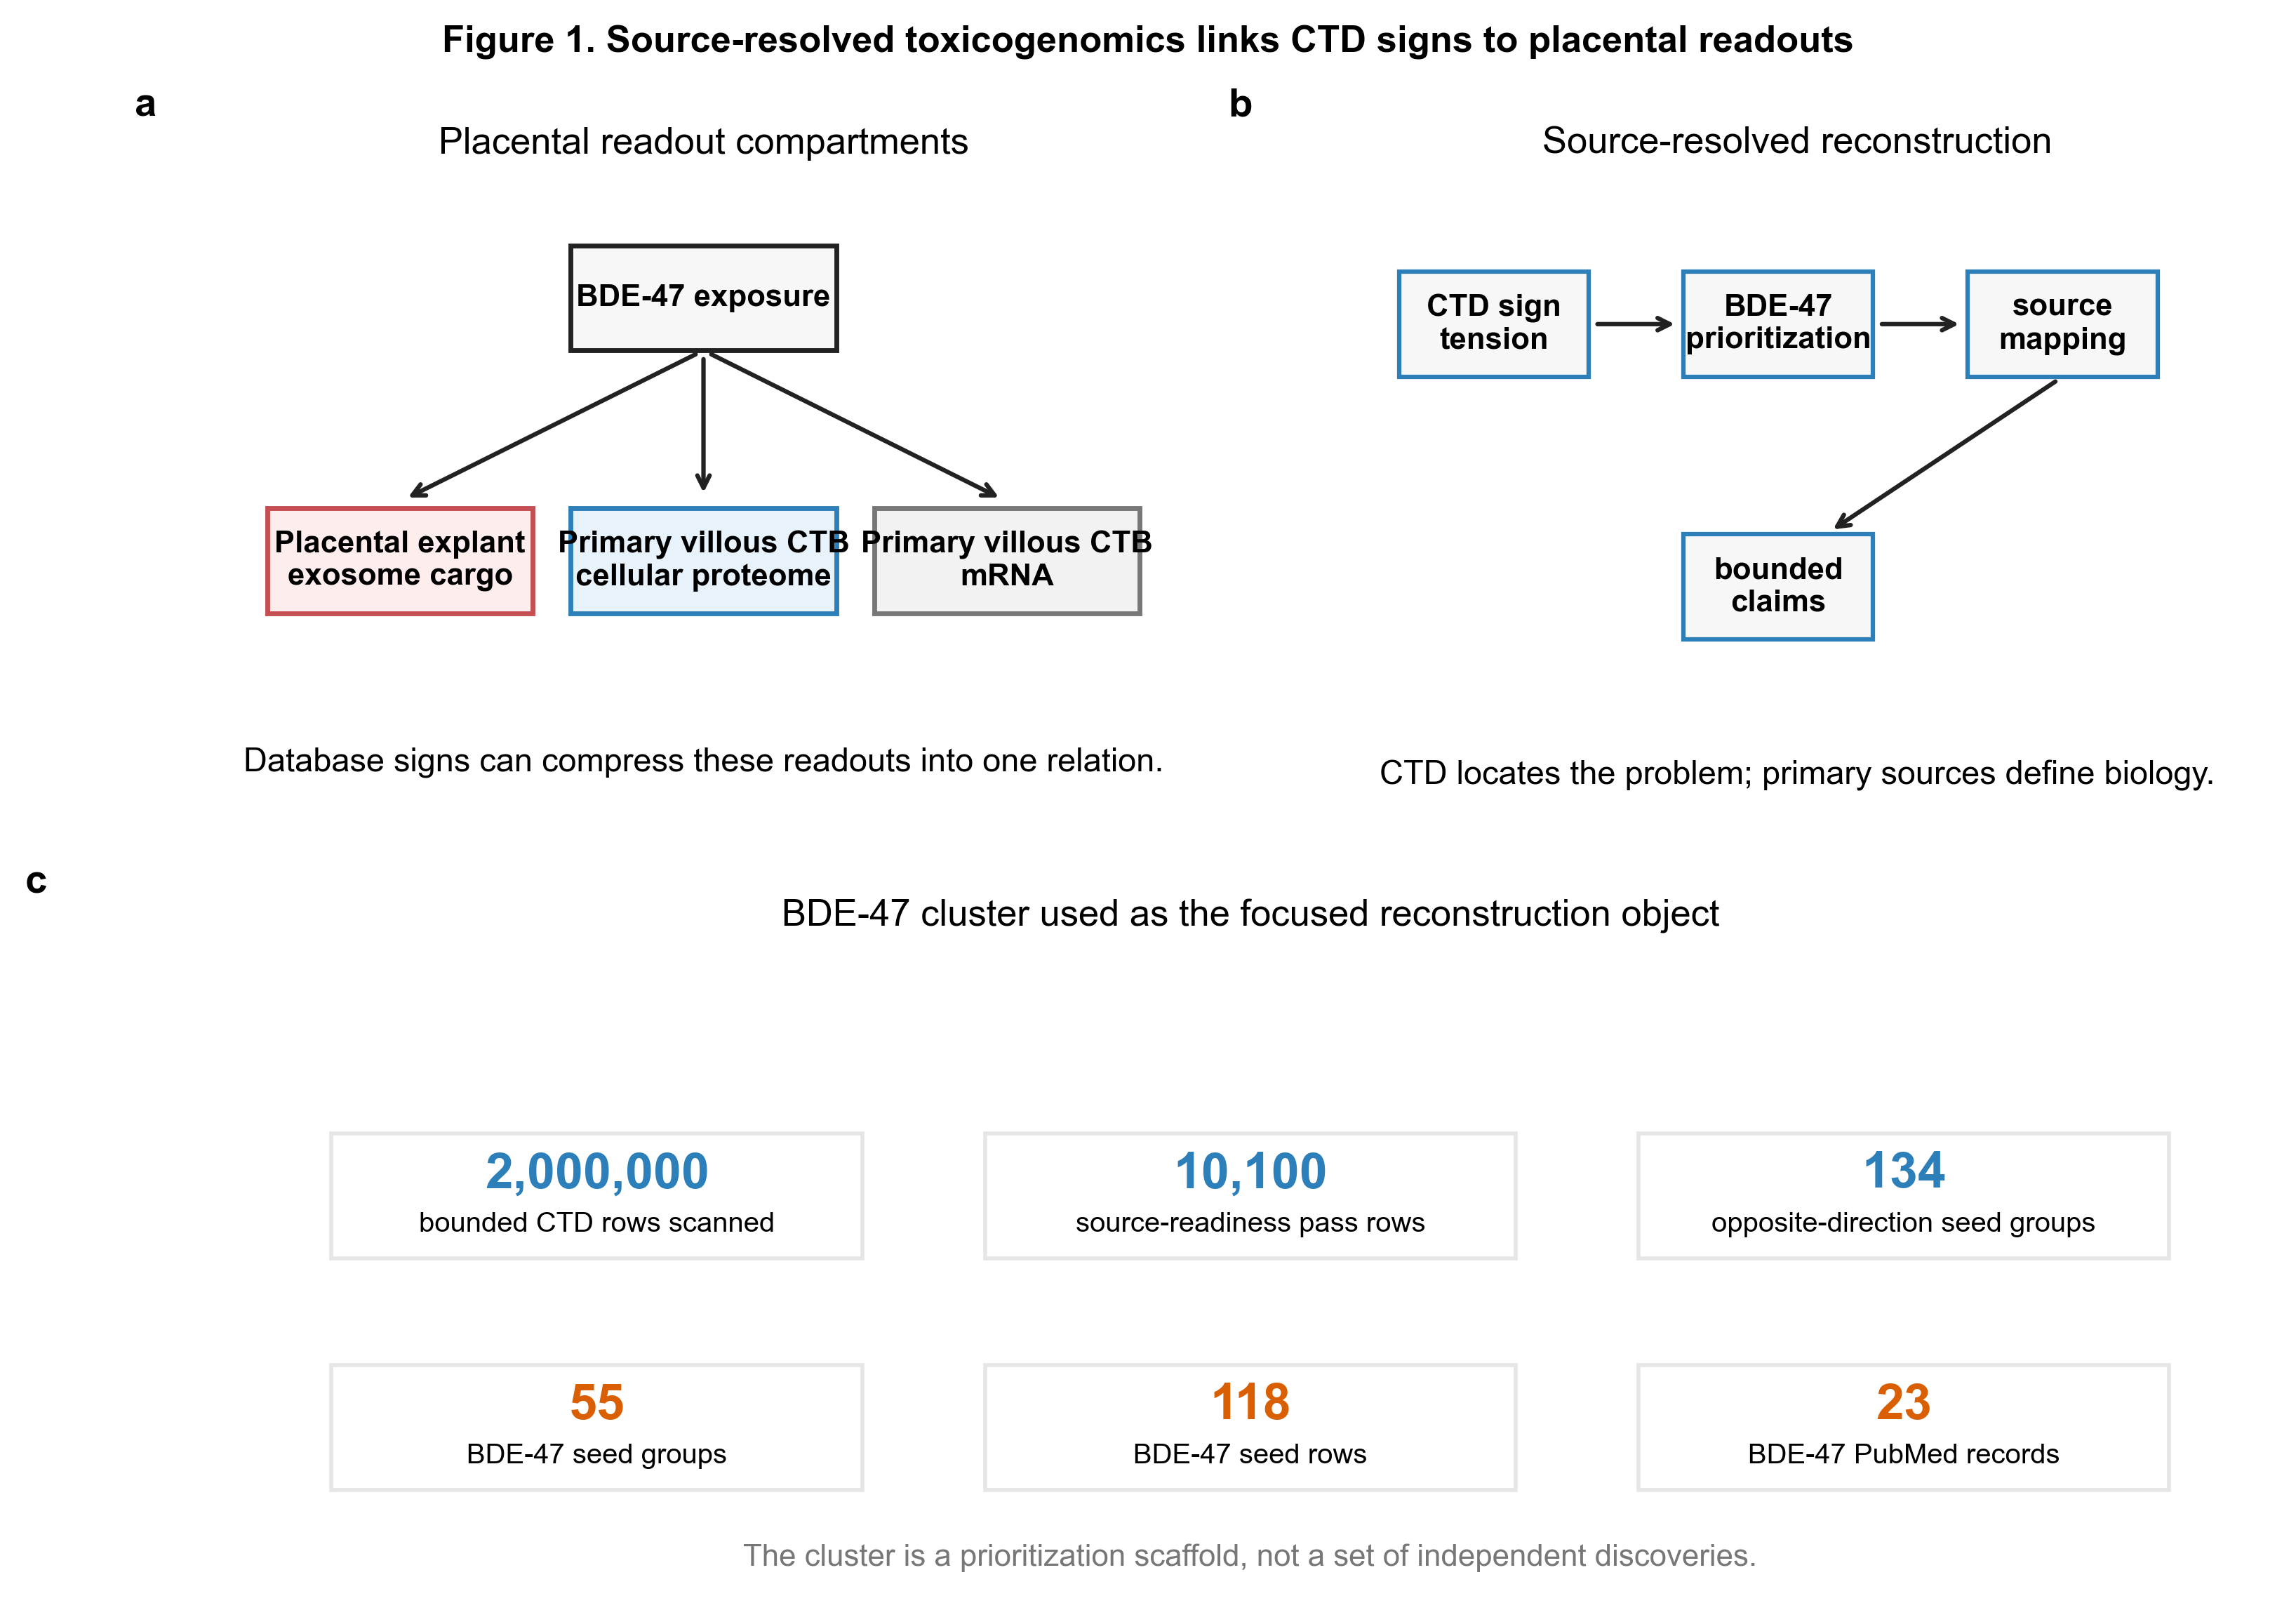
\includegraphics[width=0.96\linewidth]{figure1_commsbio_overview.png}
\caption{\textbf{Source-resolved toxicogenomics links CTD signs to placental readouts.} The study treats CTD sign tension as a prioritization scaffold and then reconstructs the source readout for BDE-47 evidence across placenta-derived exosomal cargo, primary villous cytotrophoblast cellular proteome and primary villous cytotrophoblast mRNA layers.}
\label{fig:overview}
\end{figure}

\FloatBarrier
\section{Results}

\subsection{CTD sign tension prioritizes BDE-47 for source-level reconstruction}

We built an orientation-gated CTD sign-tension graph that retained direct signed chemical-to-gene expression or activity evidence and grouped chemical-gene pairs with opposite directions. In a bounded two-million-row scan, the gate retained 10,100 source-readiness pass rows, 9,545 unique chemical-gene pairs, 134 opposite-direction seed groups and 95 independent multi-PubMed seed groups. BDE-47-like records formed the dominant local cluster, with 55 seed groups, 118 evidence rows and 23 PubMed records.

This cluster was not treated as 55 independent discoveries. It was used as a prioritization object for source-level disambiguation. A background audit supported this choice within the bounded scan: BDE-47 ranked first by opposite-direction seed count, and a within-chemical sign-label permutation that preserved BDE-47 gene row counts and sign balance gave P(count $\geq$ observed) = 0.011. These checks reduce the simplest coverage-bias explanation, but they do not replace a complete CTD-wide coverage model.

\subsection{The largest apparent BDE-47 decrease block is placenta-derived exosomal cargo}

The largest BDE-47 anchor was PMID 31675489 \cite{sheller2020}. In CTD, rows from this record appear as protein-expression evidence. Full-text and supplement inspection showed that the relevant readout is placenta-derived exosomal protein cargo from PBDE47-treated placental explants. We use PBDE47 here when referring to the treatment label in the source supplement. This reclassification changes the biological interpretation: the evidence does not demonstrate intracellular protein downregulation for this block, but decreased representation or remodeling of proteins in exosomal cargo.

All 35 CTD-mapped proteins from PMID 31675489 were recovered in the published PBDE47 supplement fold-change table. Their directions were 35/35 concordant with CTD signs, with 32 decreases and 3 increases. Seven listed zero-fold-change rows were retained as reported zero-FC entries and were not interpreted as complete biological absence. The supplement supports fold-change direction and compartment assignment, not individual protein significance, because per-protein author-level p-values or FDR were not available.

The 32-protein decreased-representation block was biologically organized. It included immune and antiviral proteins, vesicle and sorting proteins, cell-cycle and DNA-repair proteins, metabolism and translation proteins, autophagy or stress proteins, matrix and signalling proteins, and RNA processing proteins. These annotations are used as functional organization, not as a standalone enrichment claim.

\begin{figure}[H]
\centering
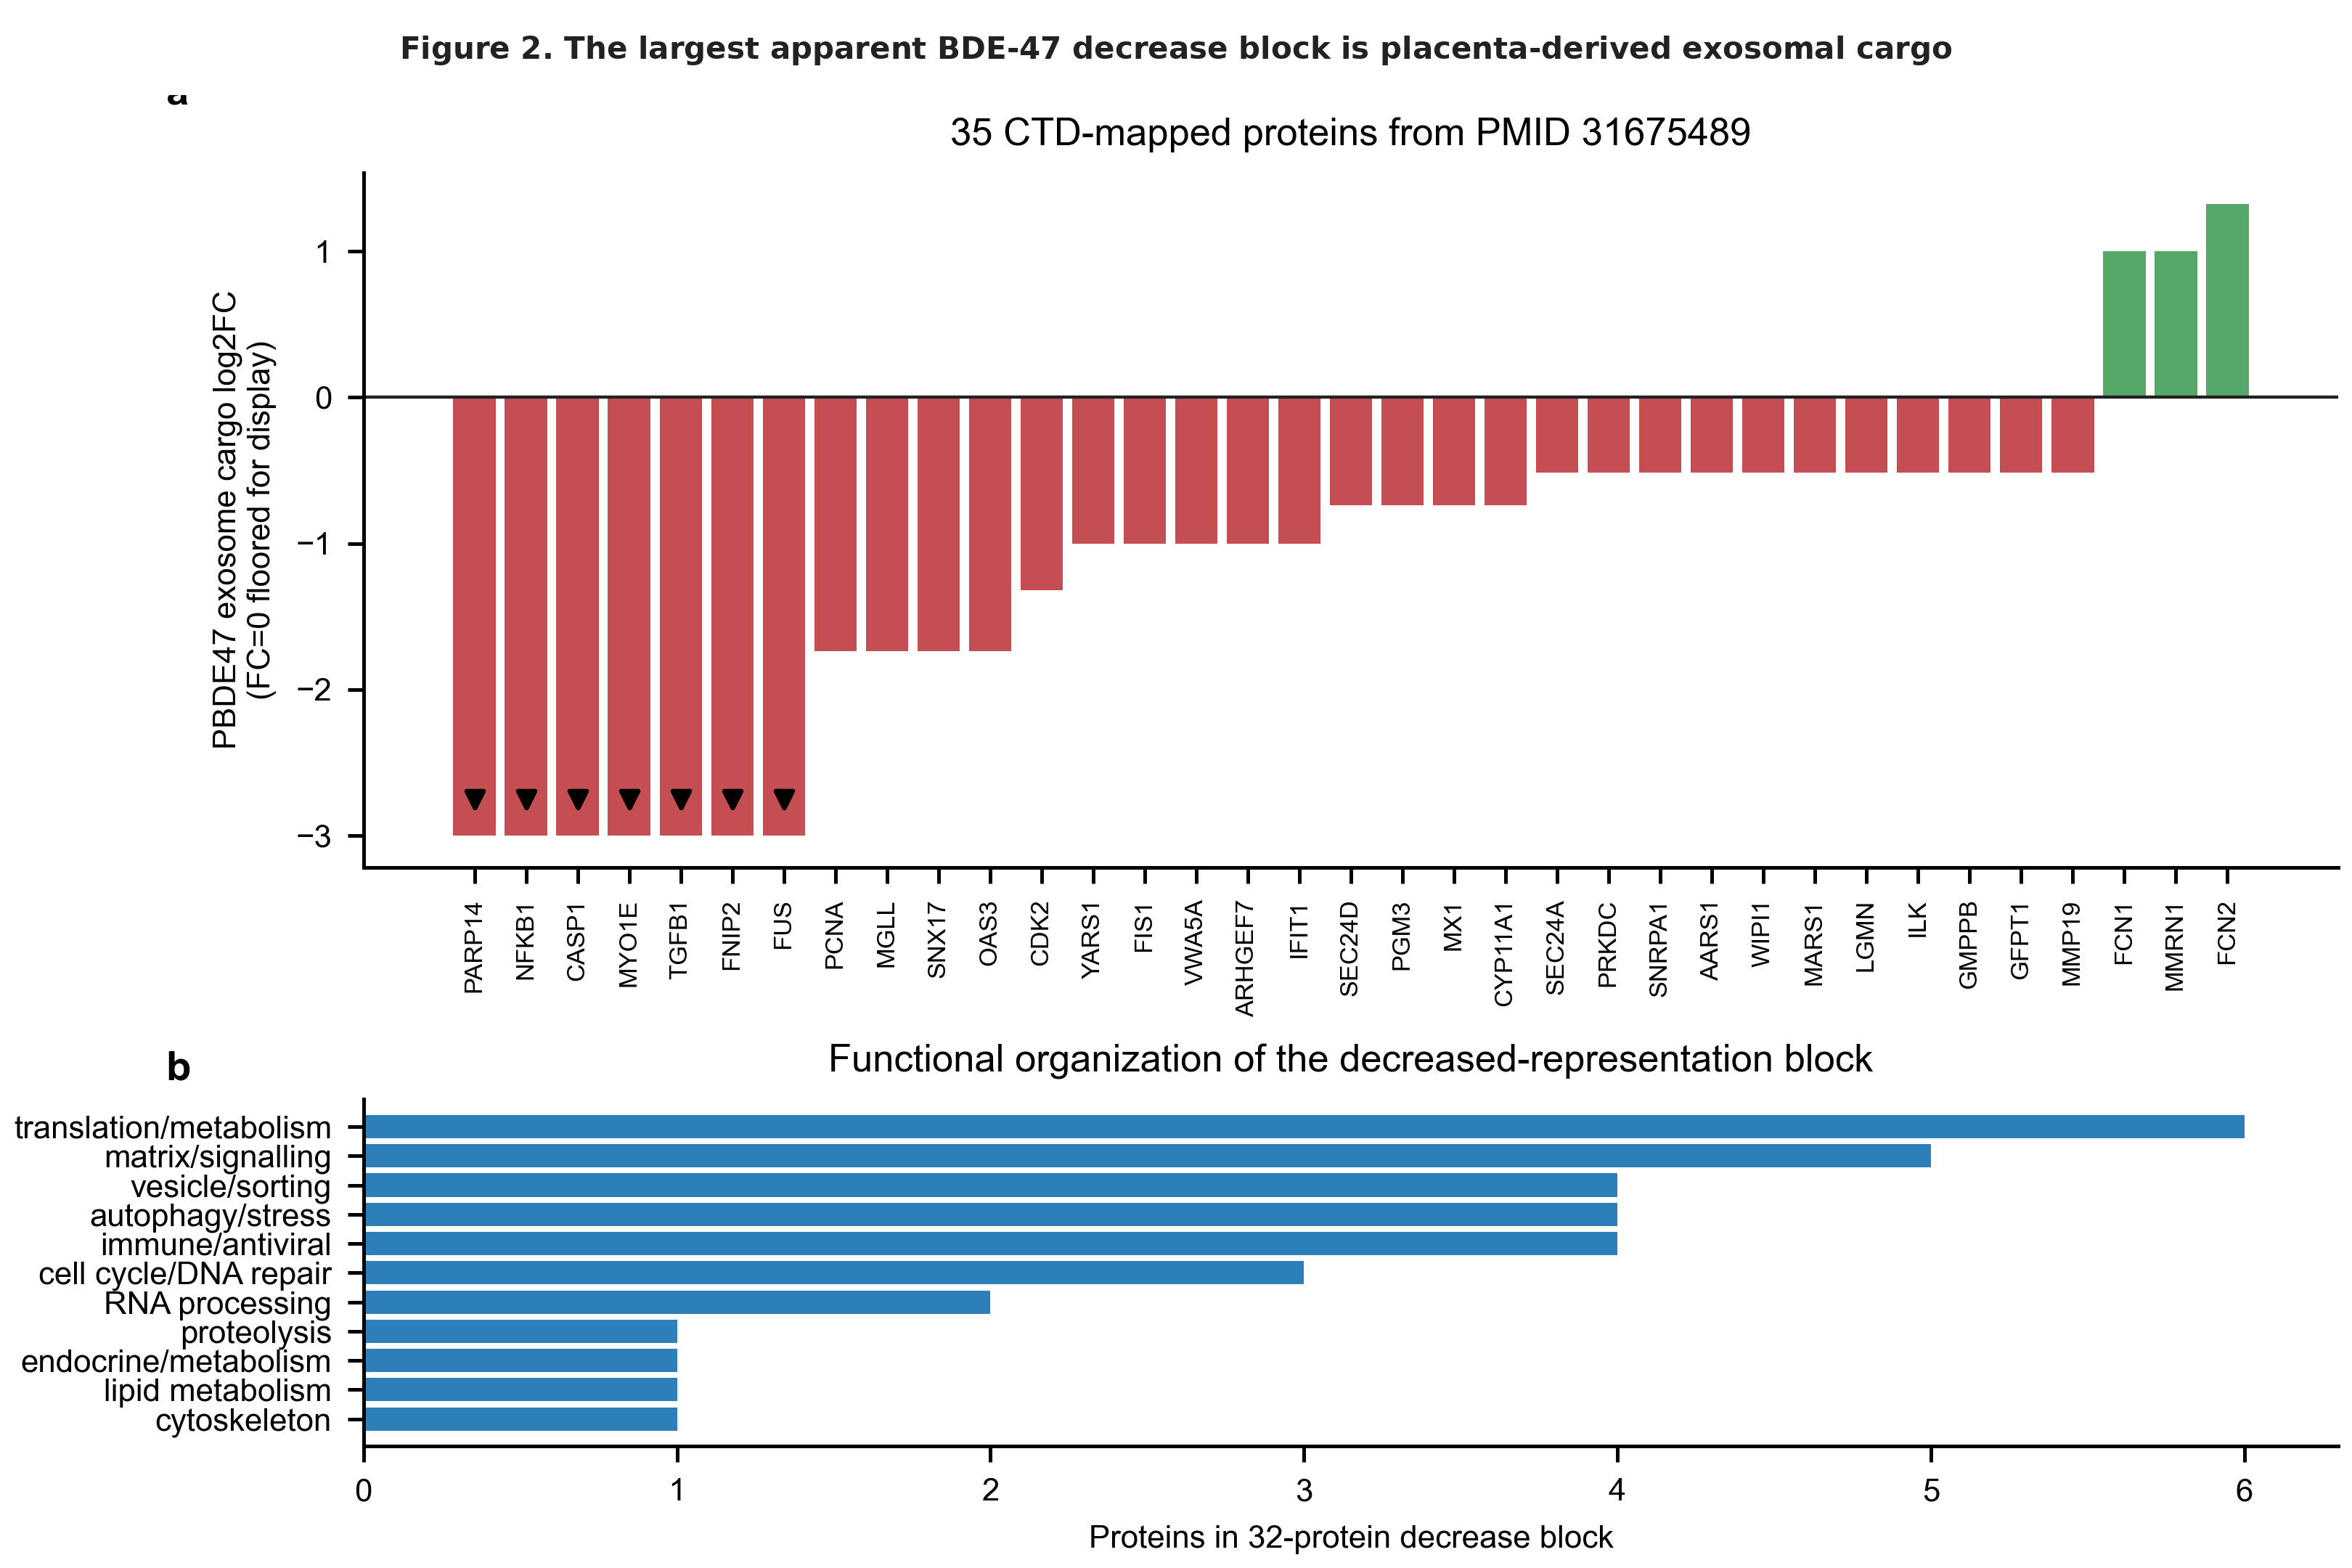
\includegraphics[width=0.96\linewidth]{figure2_exosome_cargo_block.png}
\caption{\textbf{The largest apparent BDE-47 decrease block is placenta-derived exosomal cargo.} The PMID 31675489 block contains 35 CTD-mapped proteins recovered from the PBDE47 supplement. Directions are fold-change concordant with CTD signs, but no per-protein author-level p-value or FDR claim is made.}
\label{fig:exosome}
\end{figure}

\subsection{Exosome cargo and cytotrophoblast proteome show a compact compartment contrast}

We next compared the exosome-cargo block with primary villous cytotrophoblast proteome evidence from PMID 37385330 \cite{chen2023}. Of the 35 CTD-mapped proteins from PMID 31675489, 28 were recovered in PMID 37385330 Table S1. The main contrast was restricted by a transparent protein selection tree: membership in the 31675489 exosome-cargo block, decreased exosome-cargo representation, recovery in 37385330 Table S1, CTD mapping in PMID 37385330, all-six-up direction across the six Table S1 BDE-47 conditions and bounded raw-pilot direction recovery.

ILK, NFKB1 and SNX17 satisfied this rule and define the compact CTD-supported compartment contrast. Each showed decreased representation in the PMID 31675489 exosome-cargo table but higher mean primary villous cytotrophoblast proteome abundance across all six BDE-47 dose-time conditions in PMID 37385330 Table S1. Only 227 of 3,024 Table S1 proteins were higher than vehicle mean in all six conditions. ILK, NFKB1 and SNX17 all fell into this all-six-up class, giving a descriptive hypergeometric directional-rarity check of 0.000417833. MGLL also met the directional and raw-pilot criteria but lacks PMID 37385330 CTD mapping, so it is retained as supplementary support.

To test whether the compact Table S1 direction could be recovered from raw data, we performed a bounded DIA-NN 1.8.1 library-free pilot on the strongest signal condition, BDE-47 5~\microM{}, 39 h versus vehicle 39 h \cite{demichev2020}. The pilot recovered ILK, NFKB1, SNX17 and supplementary MGLL and preserved the BDE-47-greater-than-vehicle direction for all four targets. The reconstructed log2 deltas were 0.139 for ILK, 0.138 for NFKB1, 0.109 for SNX17 and 0.224 for MGLL.

The pilot is interpreted as bounded directional evidence only. It is not the authors' original limma/FDR output, not target-protein significance, not magnitude replication and not a full raw-reconstructed differential-abundance analysis. Target-only p-values were not significant. Global comparison between the DIA-NN protein-group matrix and Table S1 at the 5~\microM{}, 39 h condition found 1,296 overlapping genes, Pearson correlation 0.1209, Spearman correlation 0.2204 and direction agreement 0.5895. SNX17 remains direction-concordant but carries a replicate-missingness caveat because the pilot used two detected BDE-47 replicates and three detected vehicle replicates after missing values were left missing.

\begin{figure}[H]
\centering
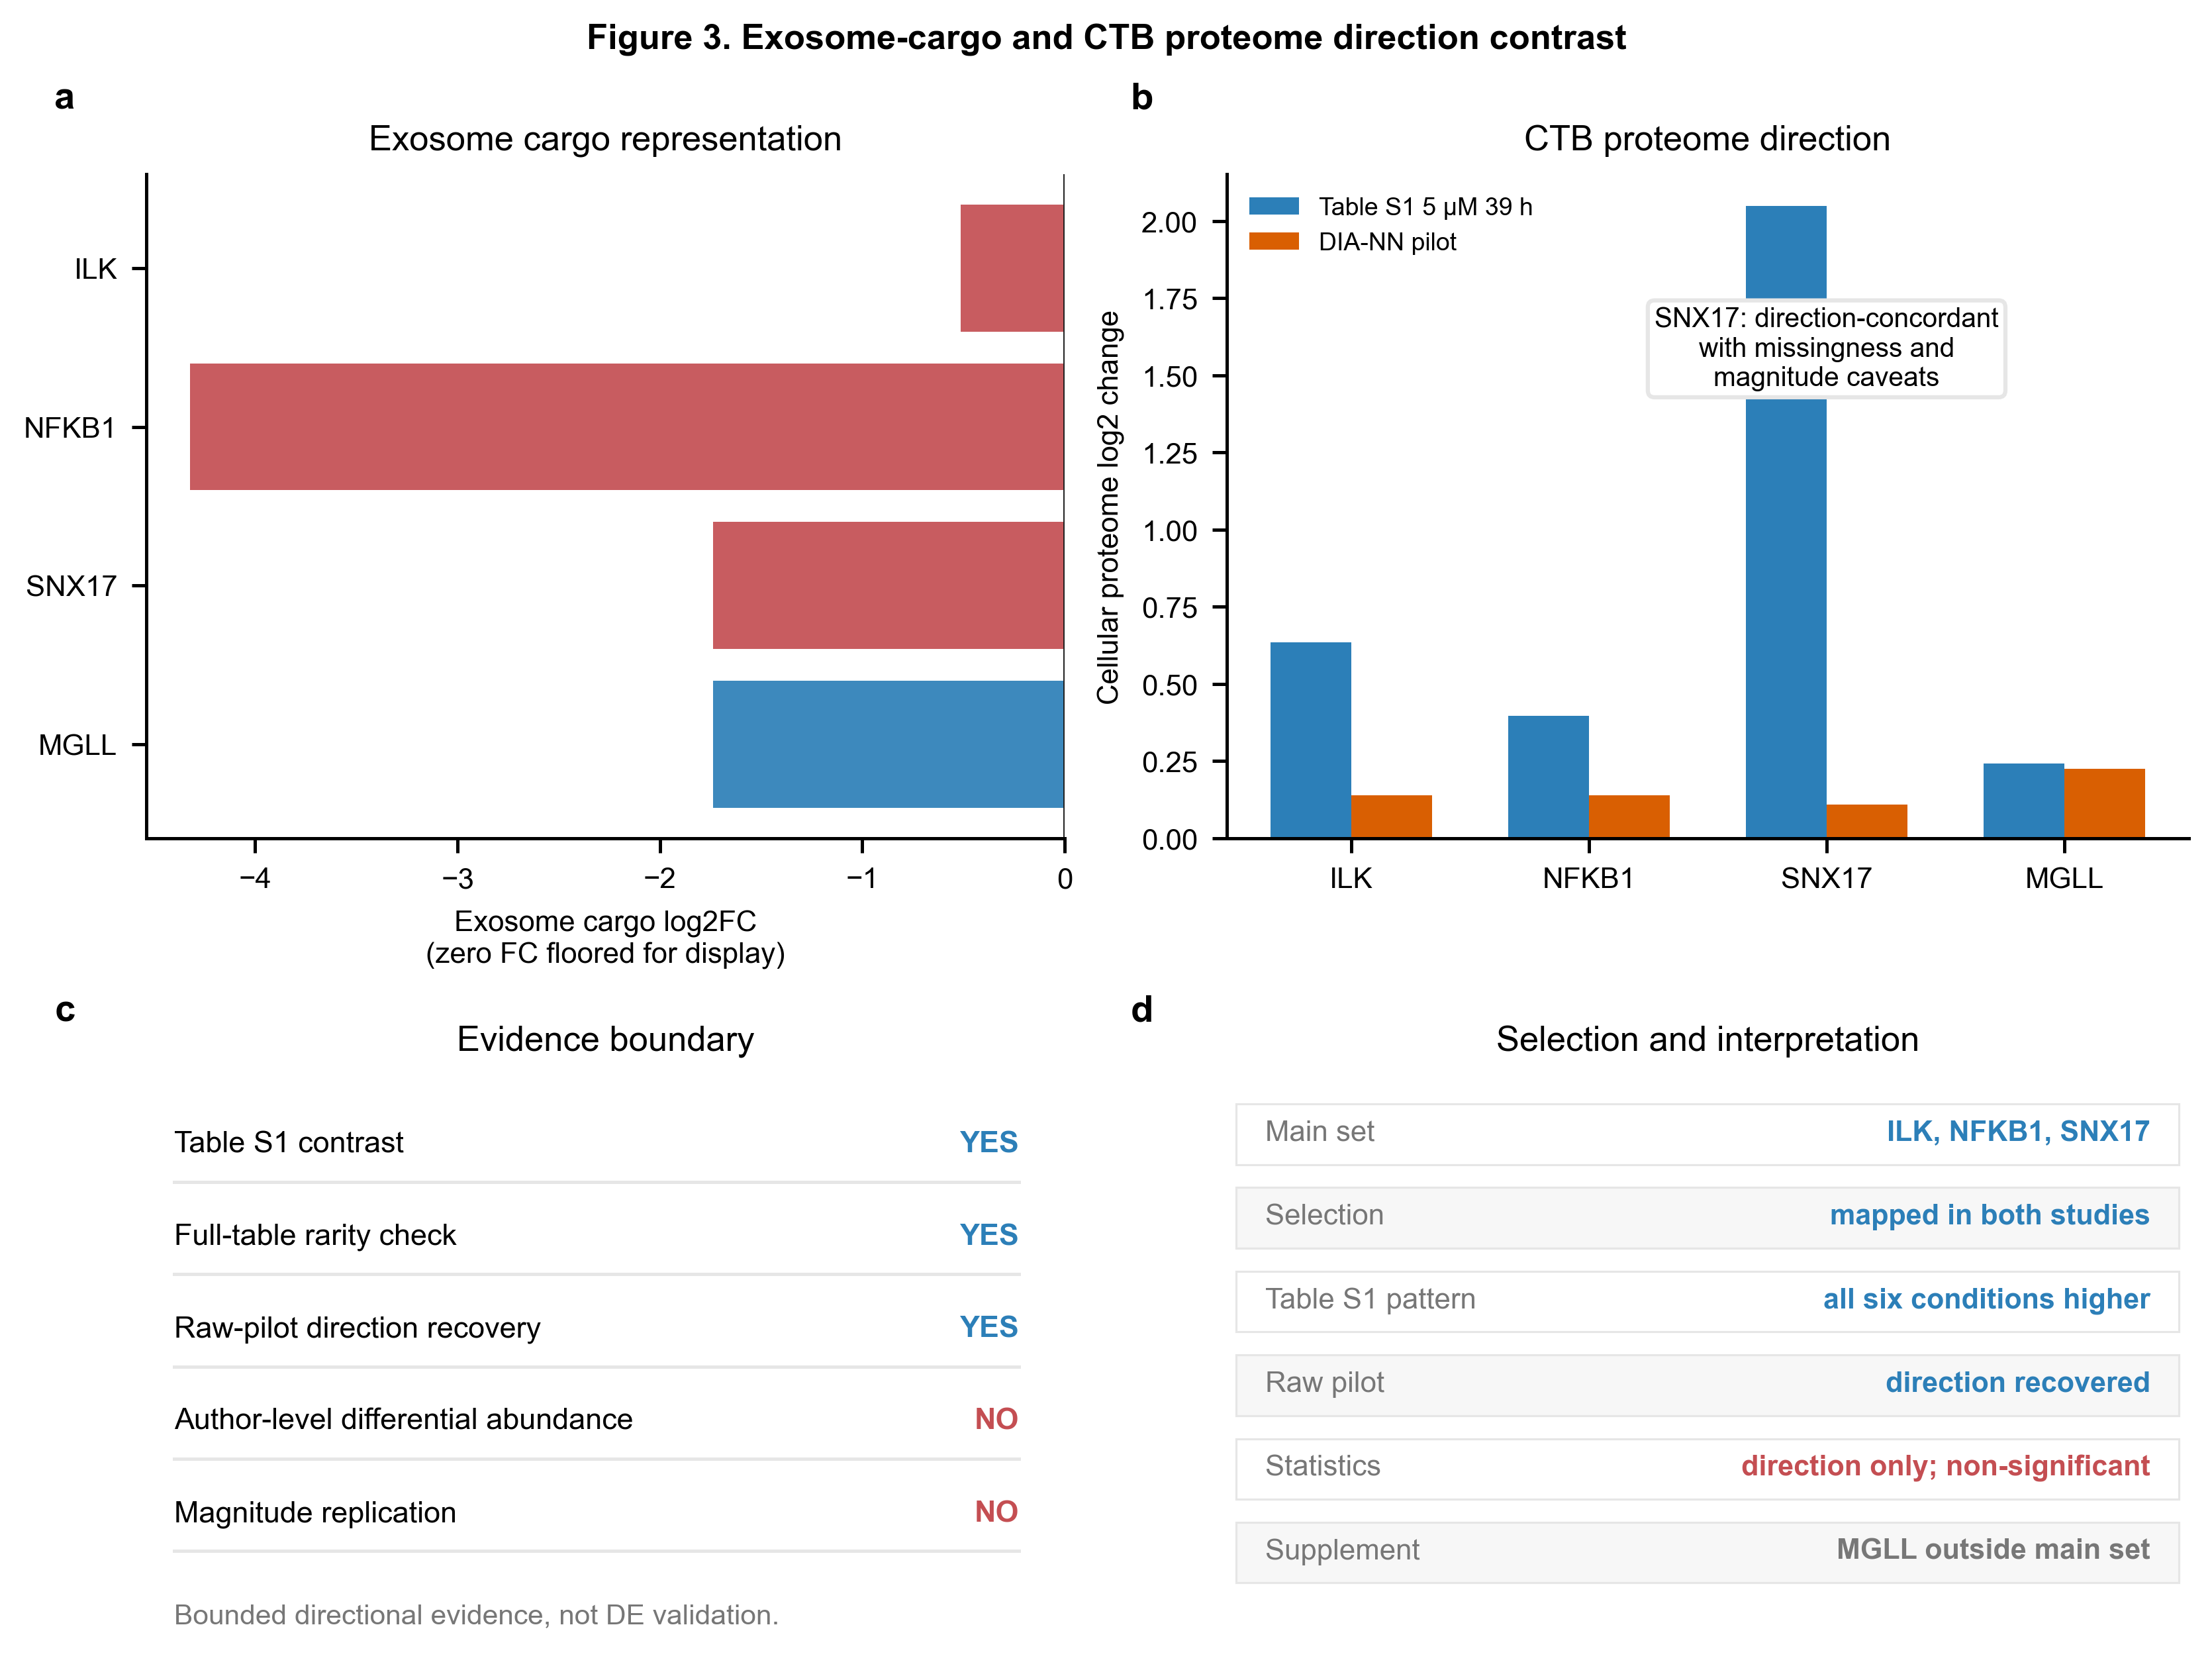
\includegraphics[width=0.96\linewidth]{figure3_compartment_contrast.png}
\caption{\textbf{Exosome cargo and CTB cellular proteome show bounded opposite directions.} ILK, NFKB1 and SNX17 show decreased representation in PMID 31675489 placenta-derived exosomal cargo but higher mean primary villous cytotrophoblast proteome abundance across six BDE-47 dose-time conditions in PMID 37385330 Table S1. A bounded DIA-NN 1.8.1 library-free reconstruction of the 5~\microM{}, 39 h raw subset recovered the same BDE-47-greater-than-vehicle direction for these targets. Raw-pilot statistics are interpreted as target-direction recovery only, not author-level limma/FDR differential abundance, target-protein significance, magnitude replication or full raw-reconstructed differential abundance. Zero fold-change values from the exosome supplement are floored only for log-scale display. SNX17 retains a replicate-missingness caveat.}
\label{fig:proteome}
\end{figure}

\subsection{Cytotrophoblast mRNA does not mirror exosome-cargo decrease}

Finally, we used GSE104896 as an independent primary villous cytotrophoblast mRNA readout check \cite{robinson2019,barrett2013}. This dataset is not an exact replication of either the exosome-cargo proteomics study or the SWATH-MS cellular proteome study. Its role is to test whether the exosome-cargo decreased-representation block is simply mirrored by uniform cellular mRNA depletion.

It was not. Among the 31675489 exosome-cargo decrease genes with non-zero paired CTB mRNA deltas, the positive mRNA fraction was 0.677, compared with a matched-null mean of 0.504. The mean log2 delta was 0.048, compared with a matched-null mean of 0.005. A donor-paired exact sign-flip model added gene-level p/FDR boundaries, and no CTD-mapped gene passed all-background BH-FDR < 0.05. We therefore use GSE104896 as a boundary analysis: decreased exosomal cargo representation is not mirrored by uniform cellular mRNA depletion, but the dataset does not establish individual-gene mRNA differential expression.

\begin{figure}[H]
\centering
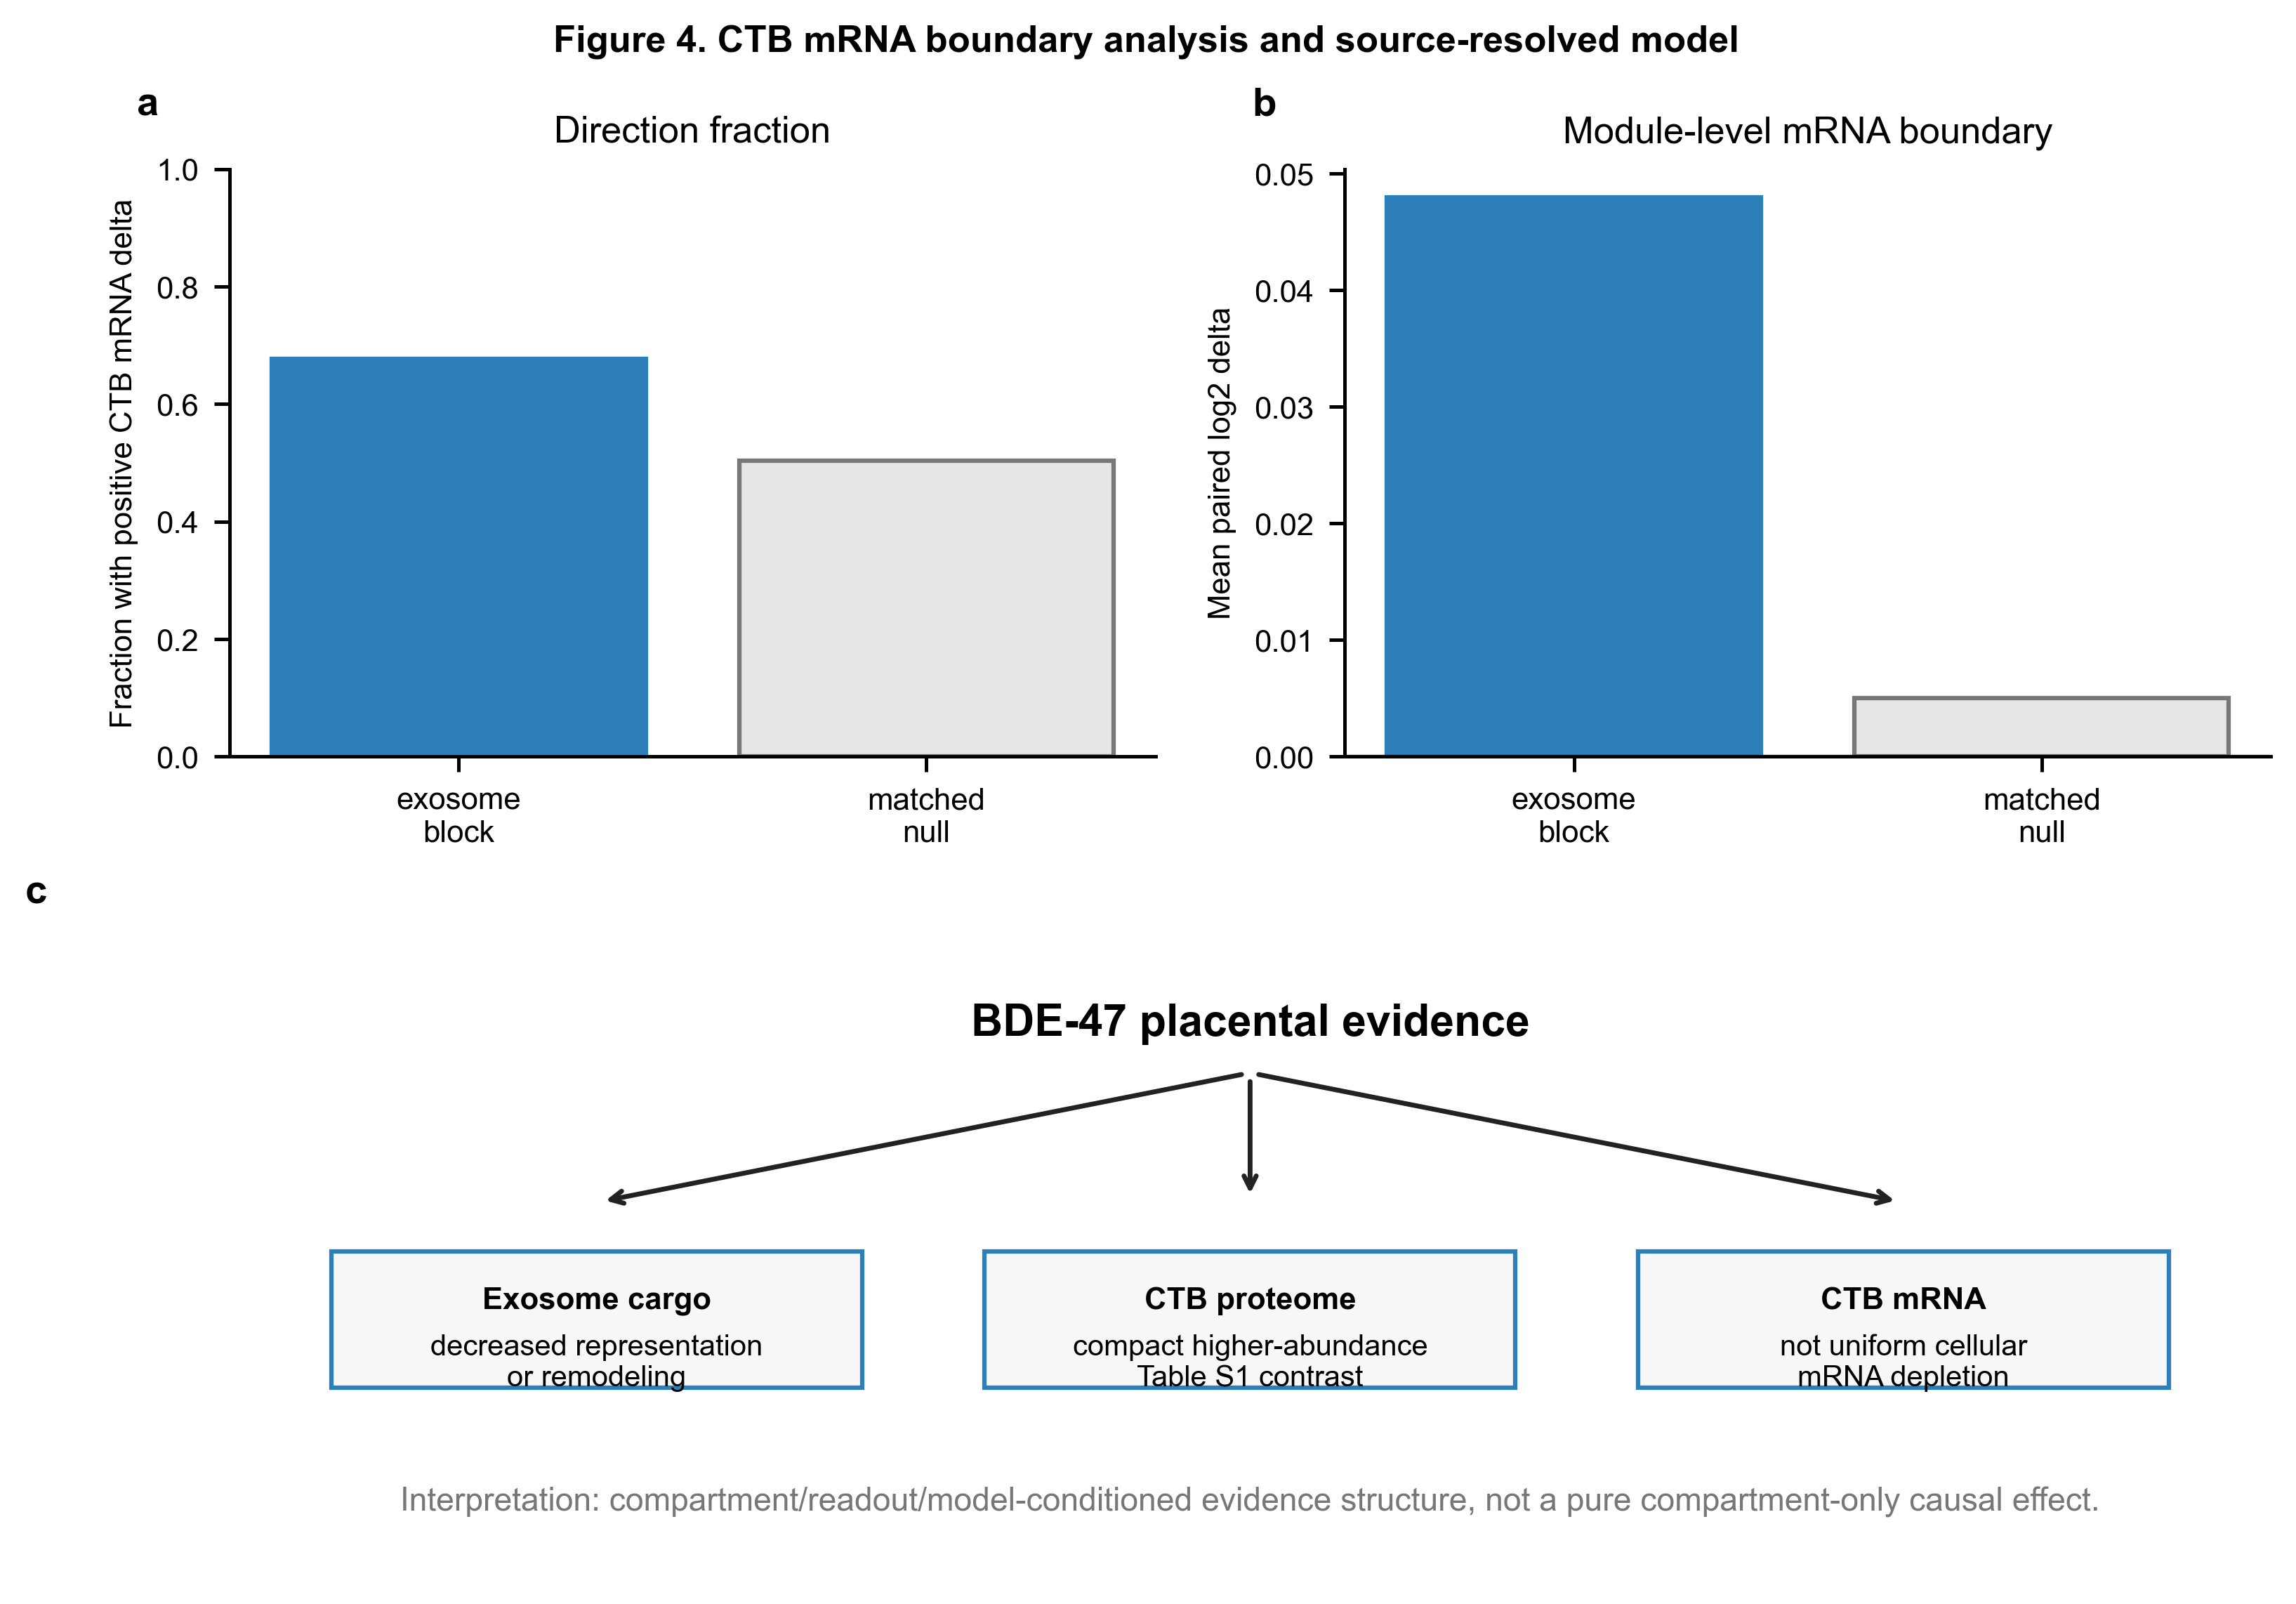
\includegraphics[width=0.96\linewidth]{figure4_mrna_model.png}
\caption{\textbf{CTB mRNA boundary analysis and source-resolved model.} GSE104896 is used as an independent mRNA boundary check, not as exact replication of the exosome-cargo or SWATH-MS proteome layers. The working model is compartment/readout/model-conditioned evidence structure, not a pure compartment-only causal claim.}
\label{fig:mrna-model}
\end{figure}

\section{Discussion}

This study reframes a BDE-47 toxicogenomic sign conflict as a source-resolved placental compartment problem. The central observation is not that BDE-47 universally increases or decreases a fixed set of proteins. Rather, the same broad database sign vocabulary can compress different biological readouts: placenta-derived exosomal cargo, primary cytotrophoblast cellular proteome and cellular mRNA. Returning to primary sources showed that the largest apparent decrease block reflects exosomal cargo representation, while selected overlapping cellular proteome and mRNA readouts do not simply mirror that decrease.

This result adds a biological interpretation to what might otherwise be treated as a database contradiction. In placenta-related toxicogenomics, extracellular vesicle cargo should not be read as a passive proxy for intracellular expression. Selective cargo representation, vesicle biogenesis, sample preparation, exposure model and cellular state can all decouple extracellular vesicle cargo from cellular proteome or transcript readouts \cite{raposo2013,vanNiel2018,thery2018}. The BDE-47 evidence block therefore supports a source-resolved model in which database sign tension can reveal hidden readout-compartment structure.

The result also has implications for toxicogenomic knowledge graphs. CTD was essential because it located an evidence-tension cluster at scale \cite{ctd2025}. But CTD was not the mechanism. Mechanistic interpretation required returning to source articles, supplementary proteomics tables, raw-pilot provenance, public mRNA data and claim-boundary audits. A useful next generation of chemical-gene evidence graphs would encode signs as observations layered by tissue, model, assay, molecular readout and compartment rather than as static edge properties.

The claim remains bounded. The CTD scan is a discovery scaffold; it does not provide effect size, statistical significance or mechanism. The 31675489 supplement supports exosomal-cargo fold-change direction, but not per-protein significance. The 37385330 cellular proteome contrast is based primarily on published Table S1 relative abundances, with bounded raw-pilot target-direction support. It is not author-level limma/FDR evidence. The GSE104896 analysis rejects a simple uniform mRNA-depletion explanation but does not provide individual-gene differential-expression claims for the exosome-cargo block. The strongest statistical upgrade would be the author-level per-protein limma/FDR table underlying the 203 differentially expressed proteins reported for PMID 37385330, or a same-sample matched cell-lysate versus extracellular-vesicle validation. A decisive biological validation would measure the same proteins in matched cell lysate and extracellular vesicle fractions under the same BDE-47 exposure.

\section{Methods}

\subsection{CTD sign-tension graph}
CTD chemical-gene interaction rows were analysed from the locally archived CTD Chemical-Gene Interactions table used for run \texttt{20260523T105644Z}. The scan was bounded to the first 2,000,000 non-comment rows and should not be interpreted as a full CTD census. Rows were retained when they represented direct signed chemical-to-gene expression or activity evidence, with signs derived from CTD action strings containing increases or decreases expression/activity classes. Rows without a PubMed identifier, rows without a signed direction, indirect rows and rows failing the source-readiness gate were excluded from the manuscript-facing sign-tension graph.

The chemical-to-gene orientation gate was deliberately fail-closed. A row passed only when the curated interaction sentence was compatible with the chemical acting on the gene/protein readout; obvious gene-to-chemical metabolism or activation statements were excluded. This rule is a heuristic orientation gate, not a semantic parser. Retained rows were grouped by chemical ID and gene ID. A chemical-gene pair was counted as an opposite-direction seed when both increase and decrease signed evidence were present after filtering. Independent multi-PubMed seeds required at least two PubMed records within the seed group. CTD-derived rows were used only as candidate/provenance evidence and never as effect-size or mechanism evidence.

\subsection{BDE-47 cluster background audit}
BDE-47 cluster dominance was evaluated inside the same bounded orientation-gated source-readiness table. Chemicals were ranked by opposite-direction seed-group count. A row-count-nearest background compared BDE-47 with the 20 non-BDE chemicals closest by pass-row count. A sign-label permutation was run for BDE-47 with seed 47 and 10,000 iterations: the observed BDE-47 signed labels were shuffled across BDE-47 gene row groups while preserving each gene group's row count and the overall BDE-47 sign balance. The reported permutation P value is the fraction of permutations with opposite-direction gene count greater than or equal to the observed count.

\subsection{PMID 31675489 exosome-cargo extraction}
PMID 31675489 was reviewed at the full-text and supplement level. CTD-mapped proteins were matched to entries in the PBDE47 supplement fold-change table by gene symbol and, when available, protein identifier. The readout was classified as placenta-derived exosomal protein cargo from placental explant conditioned medium, not intracellular protein expression. Direction concordance was assessed by comparing CTD signs with supplement fold-change direction. Listed zero-FC entries were retained as reported values and were not interpreted as complete biological absence. For log-scale display, zero-FC entries were floored only for visualization.

\subsection{PMID 37385330 Table S1 contrast and protein selection tree}
CTD-mapped proteins from the 31675489 block were mapped to PMID 37385330 Table S1 by gene/protein symbol. The cellular proteome contrasts were computed from published relative abundance values by comparing each BDE-47 dose-time condition with the corresponding vehicle mean. The six manuscript-facing BDE-47 conditions were 1~\microM{} 15 h, 5~\microM{} 15 h, 1~\microM{} 24 h, 5~\microM{} 24 h, 1~\microM{} 39 h and 5~\microM{} 39 h. The Figure~\ref{fig:proteome} main-text set required all of the following: 31675489 exosome-cargo membership, decreased exosome-cargo representation, recovery in Table S1, CTD mapping in PMID 37385330, all-six-up Table S1 direction and bounded raw-pilot direction recovery.

\subsection{Bounded DIA-NN raw pilot}
The raw-data route for PMID 37385330 was MassIVE MSV000087870 \cite{vizcaino2014,choi2020}. A bounded Route B pilot used only the BDE-47 5~\microM{}, 39 h subset and the vehicle 39 h subset. SCIEX WIFF/\texttt{.scan} files were handled in a Windows-compatible route and quantified with DIA-NN 1.8.1 in library-free mode \cite{demichev2020}. Seven preconverted \texttt{.wiff.dia} files were included in the pilot. The search used a human UniProt SwissProt FASTA downloaded on 2026-05-24, and DIA-NN generated the predicted library with \texttt{--fasta-search} and \texttt{--predictor}. Target extraction used \texttt{report.pg\_matrix.tsv} protein-group quantities. Missing values were left missing and reported through detection counts. Target-only exact p-values were descriptive and were not interpreted as global proteome FDR.

\subsection{GSE104896 mRNA boundary analysis}
GSE104896 was used as an independent primary villous cytotrophoblast mRNA readout \cite{barrett2013,robinson2019}. Probe-level records were mapped to gene symbols using the platform annotation available in the processed GEO record and collapsed to a representative gene-level value by the selected probe used in the local analysis. Paired BDE-47 versus vehicle deltas were computed by donor where pairing metadata were available. An expression-matched background permutation matched genes by selected-probe mean expression, expression standard deviation, paired-delta standard deviation and probe count. A donor-paired exact sign-flip model with all-background Benjamini-Hochberg FDR was used to define gene-level statistical boundaries.

\subsection{Use of AI-assisted tools}
AI-assisted tools were used to support code drafting, manuscript editing, figure-label checking and evidence-boundary summarization. All analyses, source mappings, statistical outputs, figure interpretations and final claims were reviewed and approved by the human authors. AI tools were not treated as authors and were not used as a source of unverified factual claims.

\section{Data availability}
This study reuses public secondary datasets and generates derived tables needed to reproduce the analyses. CTD Chemical-Gene Interaction records are available from CTD (\url{https://ctdbase.org}). PMID 31675489 and its exosome proteomics supplements are available through the published article record. PMID 37385330 is available through PubMed and \emph{Toxicology}; raw chromatograms are deposited in MassIVE under accession MSV000087870 and normalized relative abundances are provided by the source article as Table S1. GSE104896 is available from NCBI GEO. Derived tables, claim-boundary audits, proteome QC outputs, figure source data, LaTeX source and the pre-submission manuscript package are available in the public GitHub repository \url{https://github.com/Li-Hongmin/bde47-source-resolved-toxicogenomics} at release tag \texttt{v1.0-commsbio-prep} (\url{https://github.com/Li-Hongmin/bde47-source-resolved-toxicogenomics/releases/tag/v1.0-commsbio-prep}). A DOI-bearing archival snapshot will be deposited through Zenodo before final journal submission.

\section{Code availability}
Custom code used to generate the CTD sign-tension scaffold, source-level mapping tables, proteome contrast analyses, GSE104896 mRNA boundary analysis and manuscript figures is available at \url{https://github.com/Li-Hongmin/bde47-source-resolved-toxicogenomics} and release tag \texttt{v1.0-commsbio-prep}. The DIA-NN raw pilot used DIA-NN 1.8.1 and produced \texttt{report.pg\_matrix.tsv}; raw-pilot software versions and available command/parameter provenance are summarized in Supplementary Note 8. A DOI-bearing Zenodo archive of the public release will be added before final journal submission.

\section{Acknowledgements}
We thank the maintainers of CTD, GEO and MassIVE, and the authors of the source studies whose public data and supplementary materials enabled this evidence reconstruction.

\section{Author contributions}
H.L. conceived the evidence-reconstruction analysis, built the CTD sign-tension scaffold, performed source-level and computational analyses, generated figures and drafted the manuscript. B.B. contributed scientific framing, interpretation and manuscript revision. Both authors reviewed and approved the manuscript.

\section{Competing interests}
The authors declare no competing interests.

\begin{thebibliography}{99}
\bibitem{raposo2013} Raposo, G. \& Stoorvogel, W. Extracellular vesicles: exosomes, microvesicles, and friends. \emph{Journal of Cell Biology} \textbf{200}, 373--383 (2013). doi:10.1083/jcb.201211138.
\bibitem{vanNiel2018} van Niel, G., D'Angelo, G. \& Raposo, G. Shedding light on the cell biology of extracellular vesicles. \emph{Nature Reviews Molecular Cell Biology} \textbf{19}, 213--228 (2018). doi:10.1038/nrm.2017.125.
\bibitem{thery2018} Thery, C. et al. Minimal information for studies of extracellular vesicles 2018 (MISEV2018). \emph{Journal of Extracellular Vesicles} \textbf{7}, 1535750 (2018). doi:10.1080/20013078.2018.1535750.
\bibitem{burkova2021} Burkova, E. E., Sedykh, S. E. \& Nevinsky, G. A. Human placenta exosomes: biogenesis, isolation, composition, and prospects for use in diagnostics. \emph{International Journal of Molecular Sciences} \textbf{22}, 2158 (2021). doi:10.3390/ijms22042158.
\bibitem{nishi2024} Nishi, K. \& Modi, D. Placental exosomes in pregnancy and preeclampsia. \emph{American Journal of Reproductive Immunology} \textbf{91}, e13857 (2024). doi:10.1111/aji.13857.
\bibitem{herbstman2010} Herbstman, J. B. et al. Prenatal exposure to PBDEs and neurodevelopment. \emph{Environmental Health Perspectives} \textbf{118}, 712--719 (2010). doi:10.1289/ehp.0901340.
\bibitem{ruis2023} Ruis, M., Hoffman, K. \& Stapleton, H. M. Brominated flame retardants and legacy organochlorines in archived human placenta samples: sex differences, temporal analysis and associations with infant birth weight. \emph{Chemosphere} \textbf{322}, 138170 (2023). doi:10.1016/j.chemosphere.2023.138170.
\bibitem{ouidir2020} Ouidir, M. et al. Concentrations of persistent organic pollutants in maternal plasma and epigenome-wide placental DNA methylation. \emph{Clinical Epigenetics} \textbf{12}, 103 (2020). doi:10.1186/s13148-020-00894-6.
\bibitem{robinson2019} Robinson, J. F. et al. Genomic profiling of BDE-47 effects on human placental cytotrophoblasts. \emph{Toxicological Sciences} \textbf{167}, 211--226 (2019). doi:10.1093/toxsci/kfy230.
\bibitem{chen2023} Chen, H. et al. Proteomic analyses of primary human villous trophoblasts exposed to flame retardant BDE-47 using SWATH-MS. \emph{Toxicology} \textbf{494}, 153583 (2023). doi:10.1016/j.tox.2023.153583.
\bibitem{sheller2020} Sheller-Miller, S. et al. Environmental pollutant induced cellular injury is reflected in exosomes from placental explants. \emph{Placenta} \textbf{89}, 42--49 (2020). doi:10.1016/j.placenta.2019.10.008.
\bibitem{ctd2025} Davis, A. P. et al. Comparative Toxicogenomics Database's 20th anniversary: update 2025. \emph{Nucleic Acids Research} \textbf{53}, D1328--D1334 (2025). doi:10.1093/nar/gkae883.
\bibitem{elAndaloussi2013} El Andaloussi, S., Mager, I., Breakefield, X. O. \& Wood, M. J. A. Extracellular vesicles: biology and emerging therapeutic opportunities. \emph{Nature Reviews Drug Discovery} \textbf{12}, 347--357 (2013). doi:10.1038/nrd3978.
\bibitem{gillet2012} Gillet, L. C. et al. Targeted data extraction of the MS/MS spectra generated by data-independent acquisition: a new concept for consistent and accurate proteome analysis. \emph{Molecular \& Cellular Proteomics} \textbf{11}, O111.016717 (2012). doi:10.1074/mcp.O111.016717.
\bibitem{demichev2020} Demichev, V. et al. DIA-NN: neural networks and interference correction enable deep proteome coverage in high throughput. \emph{Nature Methods} \textbf{17}, 41--44 (2020). doi:10.1038/s41592-019-0638-x.
\bibitem{ritchie2015} Ritchie, M. E. et al. limma powers differential expression analyses for RNA-sequencing and microarray studies. \emph{Nucleic Acids Research} \textbf{43}, e47 (2015). doi:10.1093/nar/gkv007.
\bibitem{barrett2013} Barrett, T. et al. NCBI GEO: archive for functional genomics data sets--update. \emph{Nucleic Acids Research} \textbf{41}, D991--D995 (2013). doi:10.1093/nar/gks1193.
\bibitem{vizcaino2014} Vizcaino, J. A. et al. ProteomeXchange provides globally coordinated proteomics data submission and dissemination. \emph{Nature Biotechnology} \textbf{32}, 223--226 (2014). doi:10.1038/nbt.2839.
\bibitem{choi2020} Choi, M. et al. MassIVE.quant: a community resource of quantitative mass spectrometry-based proteomics datasets. \emph{Nature Methods} \textbf{17}, 981--984 (2020). doi:10.1038/s41592-020-0955-0.
\bibitem{maclean2010} MacLean, B. et al. Skyline: an open source document editor for creating and analyzing targeted proteomics experiments. \emph{Bioinformatics} \textbf{26}, 966--968 (2010). doi:10.1093/bioinformatics/btq054.
\bibitem{bruderer2015} Bruderer, R. et al. Extending the limits of quantitative proteome profiling with data-independent acquisition and application to acetaminophen-treated three-dimensional liver microtissues. \emph{Molecular \& Cellular Proteomics} \textbf{14}, 1400--1410 (2015). doi:10.1074/mcp.M114.044305.
\bibitem{perezriverol2022} Perez-Riverol, Y. et al. The PRIDE database resources in 2022: a hub for mass spectrometry-based proteomics evidences. \emph{Nucleic Acids Research} \textbf{50}, D543--D552 (2022). doi:10.1093/nar/gkab1038.
\bibitem{mcnutt2018} McNutt, M. K. et al. Transparency in authors' contributions and responsibilities to promote integrity in scientific publication. \emph{Proceedings of the National Academy of Sciences USA} \textbf{115}, 2557--2560 (2018). doi:10.1073/pnas.1715374115.
\bibitem{deutsch2020} Deutsch, E. W. et al. The ProteomeXchange consortium in 2020: enabling big data approaches in proteomics. \emph{Nucleic Acids Research} \textbf{48}, D1145--D1152 (2020). doi:10.1093/nar/gkz984.
\bibitem{szklanna2017} Szklanna, P. B. et al. Comparative proteomic analysis of trophoblast cell models reveals their differential phenotypes, potential uses, and limitations. \emph{Proteomics} \textbf{17}, e1700037 (2017). doi:10.1002/pmic.201700037.
\end{thebibliography}

\clearpage
\appendix
\section*{Supplementary Information}
\addcontentsline{toc}{section}{Supplementary Information}

\subsection*{Supplementary Note 1. Evidence boundary definitions for Figure~\ref{fig:proteome}}
Figure~\ref{fig:proteome} is retained in the main manuscript as Level 2.5 evidence. The term means that the contrast is supported by published Table S1 relative abundances, a full-table directional-background check and a bounded DIA-NN target-direction recovery pilot. It does not mean author-level differential abundance, target-protein significance, magnitude replication or a full raw-reconstructed proteome analysis.

\begin{table}[H]
\centering
\caption{Evidence-boundary definitions for Figure~\ref{fig:proteome}.}
\begin{tabular}{p{0.14\linewidth}p{0.58\linewidth}p{0.20\linewidth}}
\toprule
Level & Definition & Status for Figure~\ref{fig:proteome} \\
\midrule
Level 1 & Published Table S1 descriptive contrast only & Passed \\
Level 2 & Table S1 contrast plus full-table directional-background check & Passed \\
Level 2.5 & Level 2 plus bounded raw-pilot target recovery and direction preservation & Current \\
Level 3 & Raw-reconstructed replicate-level differential abundance with robust target statistics & Not reached \\
Level 4 & Author-level limma/FDR table or full reproducible raw reanalysis across all conditions & Not reached \\
\bottomrule
\end{tabular}
\end{table}

\subsection*{Supplementary Note 2. CTD sign-tension scaffold}
The CTD scan was designed as a discovery scaffold. It retained direct signed chemical-to-gene rows that passed source-readiness and orientation gates. A bounded two-million-row scan yielded 10,100 source-readiness pass rows, 9,545 unique chemical-gene pairs, 134 opposite-direction seed groups and 95 independent multi-PubMed seed groups. BDE-47-like records formed the largest local cluster, with 55 seed groups, 118 evidence rows and 23 PubMed records.

\subsection*{Supplementary Note 3. PMID 31675489 exosomal-cargo reclassification}
PMID 31675489 was reclassified from broad protein-expression evidence to placenta-derived exosomal protein cargo. Thirty-five CTD-mapped proteins were recovered in the PBDE47 supplement fold-change table. All 35 directions were concordant with CTD signs, with 32 decreases and 3 increases. The supplement supports direction and compartment assignment. It does not support per-protein statistical significance.

\subsection*{Supplementary Note 4. Figure 3 protein selection tree}
The main-text Figure~\ref{fig:proteome} set is ILK, NFKB1 and SNX17. Proteins entered the main-text set only if they satisfied all of the following criteria: membership in the 31675489 CTD/supplement block, decreased exosome-cargo representation, recovery in PMID 37385330 Table S1, CTD mapping in PMID 37385330, all-six-up direction across the six Table S1 BDE-47 conditions and bounded raw-pilot direction recovery. MGLL is retained as supplementary directional support because it lacks PMID 37385330 CTD mapping despite strong direction and magnitude agreement in the raw pilot.


\subsubsection*{Supplementary Figure 1. Protein selection tree criteria.}
\begin{center}
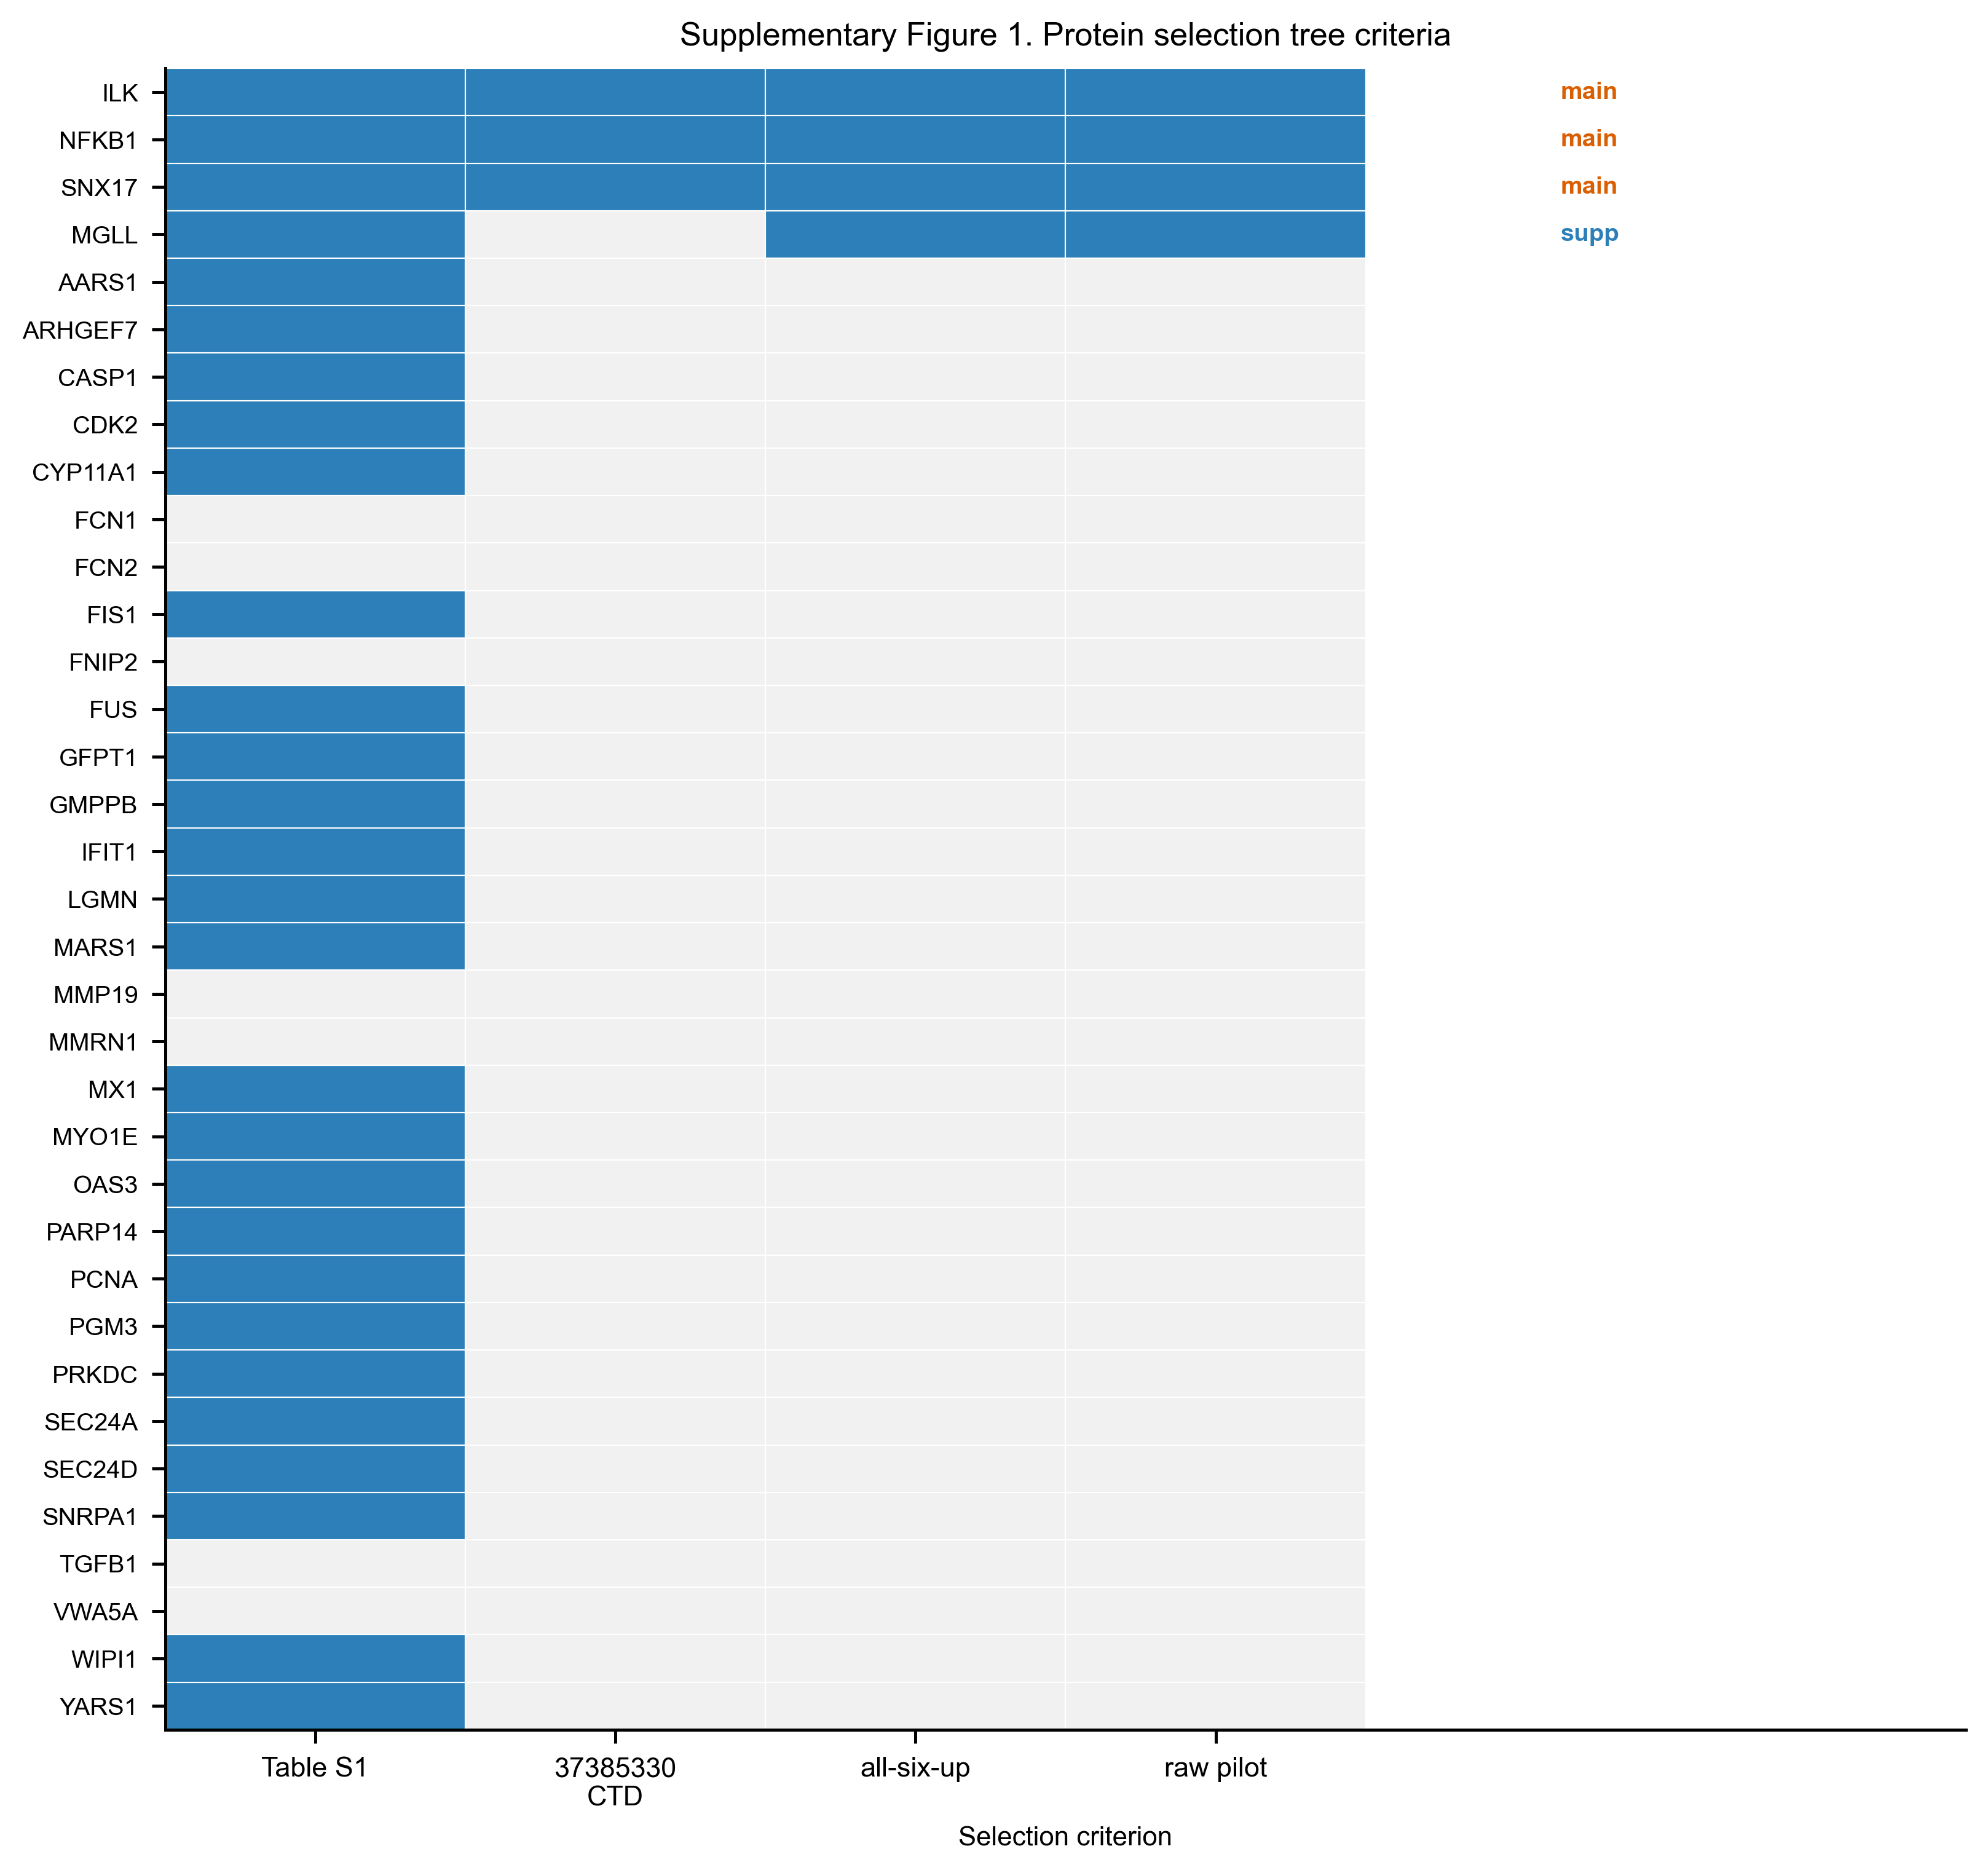
\includegraphics[width=0.95\linewidth]{suppfig1_selection_tree.png}
\end{center}


\subsection*{Supplementary Note 5. Figure 3 Table S1 and raw-pilot boundary}
In PMID 37385330 Table S1, ILK, NFKB1 and SNX17 were higher than the vehicle mean in all six BDE-47 dose-time contrasts. Across the full Table S1 background, 227 of 3,024 proteins were all-six-up. The three-target directional-rarity check was 0.000417833. The broader 28-protein overlap did not show strong all-six-up enrichment (P = 0.153979), so the manuscript keeps the claim compact.

The bounded DIA-NN 1.8.1 raw pilot used only the BDE-47 5~\microM{}, 39 h subset and vehicle 39 h subset. It recovered ILK, NFKB1, SNX17 and MGLL with BDE-47-greater-than-vehicle direction. However, target-only p-values were non-significant and raw-pilot effect sizes were smaller than Table S1 contrasts. Global pg-matrix agreement with Table S1 was modest: 1,296 overlapping genes, Pearson 0.1209, Spearman 0.2204 and direction agreement 0.5895. SNX17 is direction-concordant but carries a replicate-missingness caveat.

\begin{table}[H]
\centering
\caption{Target-level raw-pilot boundary.}
\scriptsize
\begin{tabular}{p{0.08\linewidth}p{0.20\linewidth}p{0.13\linewidth}p{0.13\linewidth}p{0.11\linewidth}p{0.22\linewidth}}
\toprule
Gene & Use & Table S1 log2FC & Raw log2 delta & Target p & Detection \\
\midrule
ILK & Main & 0.633637 & 0.139289 & 0.48571429 & 3/3 BDE; 4/4 vehicle \\
NFKB1 & Main & 0.396524 & 0.137800 & 0.37142857 & 3/3 BDE; 4/4 vehicle \\
SNX17 & Main; missingness caveat & 2.048821 & 0.108717 & 0.90000000 & 2/3 BDE; 3/4 vehicle \\
MGLL & Supplementary & 0.242264 & 0.223915 & 0.62857143 & 3/3 BDE; 4/4 vehicle \\
\bottomrule
\end{tabular}
\end{table}


\subsubsection*{Supplementary Figure 2. Raw pilot versus Table S1 global QC.}
\begin{center}
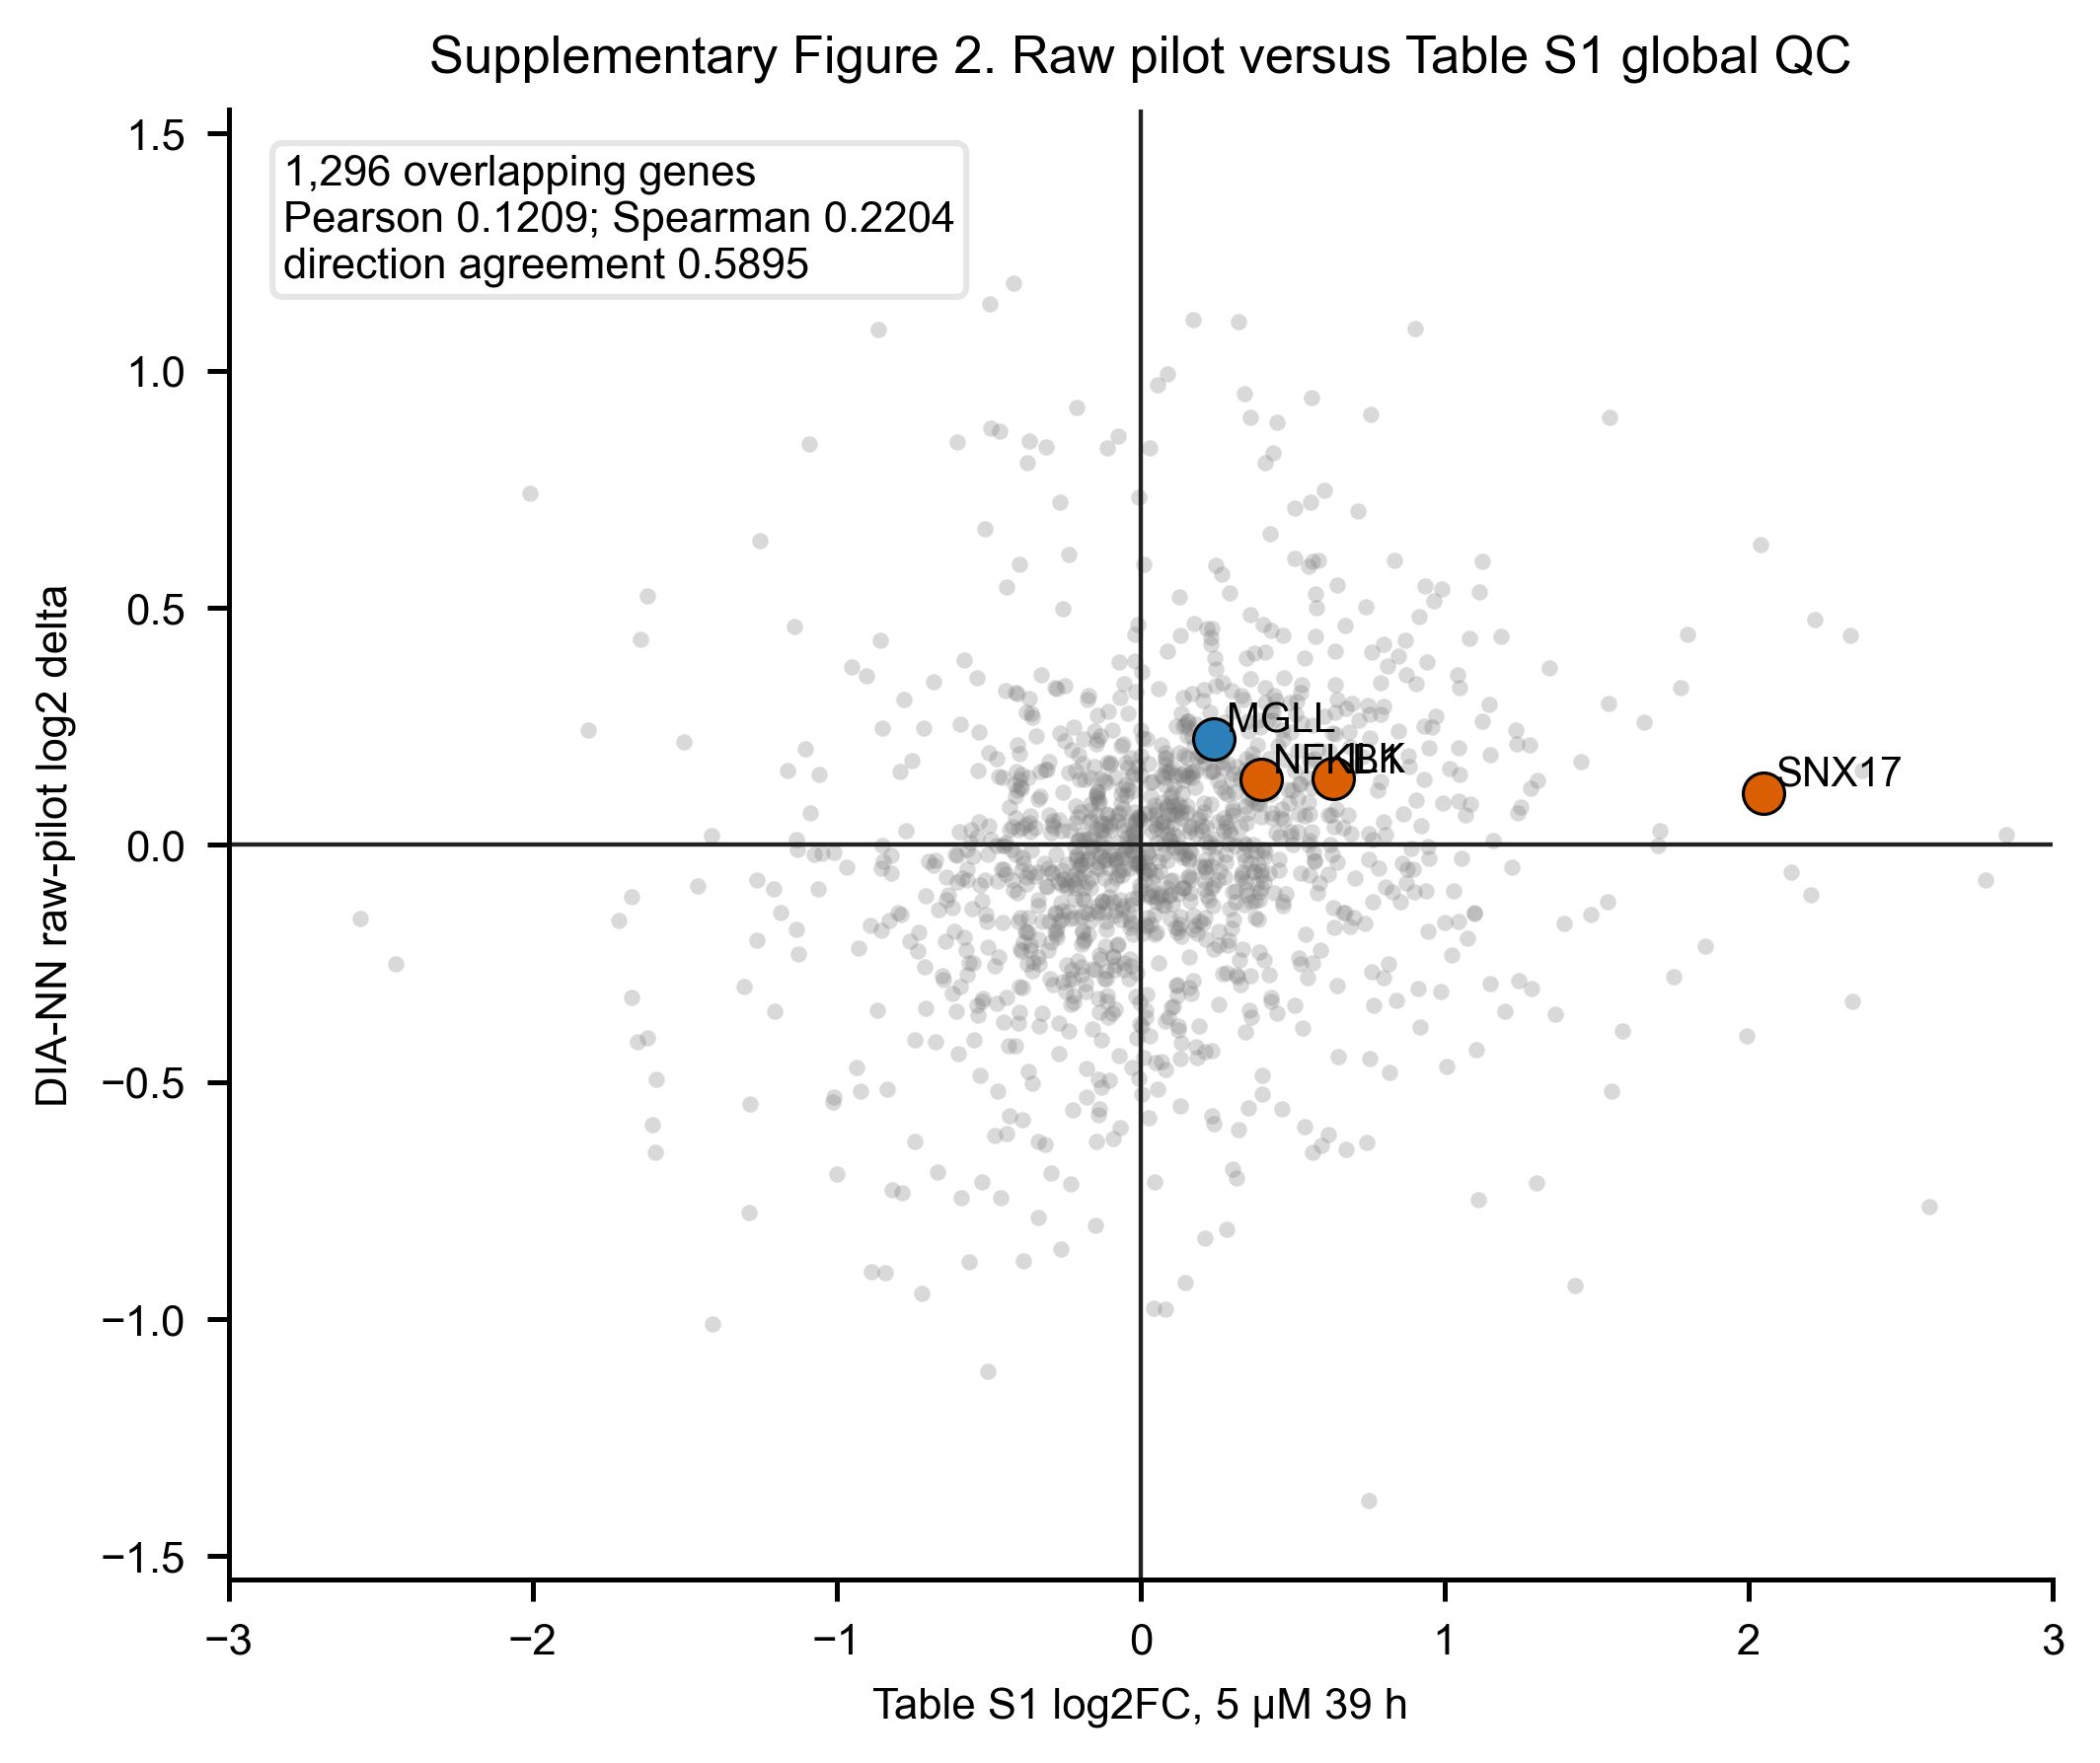
\includegraphics[width=0.82\linewidth]{suppfig2_raw_vs_table_s1.png}
\end{center}
\noindent\textit{Grey points show all 1,296 genes overlapping between Table S1 and the DIA-NN protein-group matrix; highlighted targets are ILK, NFKB1, SNX17 and supplementary MGLL.}



\subsubsection*{Supplementary Figure 3. Target magnitude agreement is insufficient for Level 3.}
\begin{center}
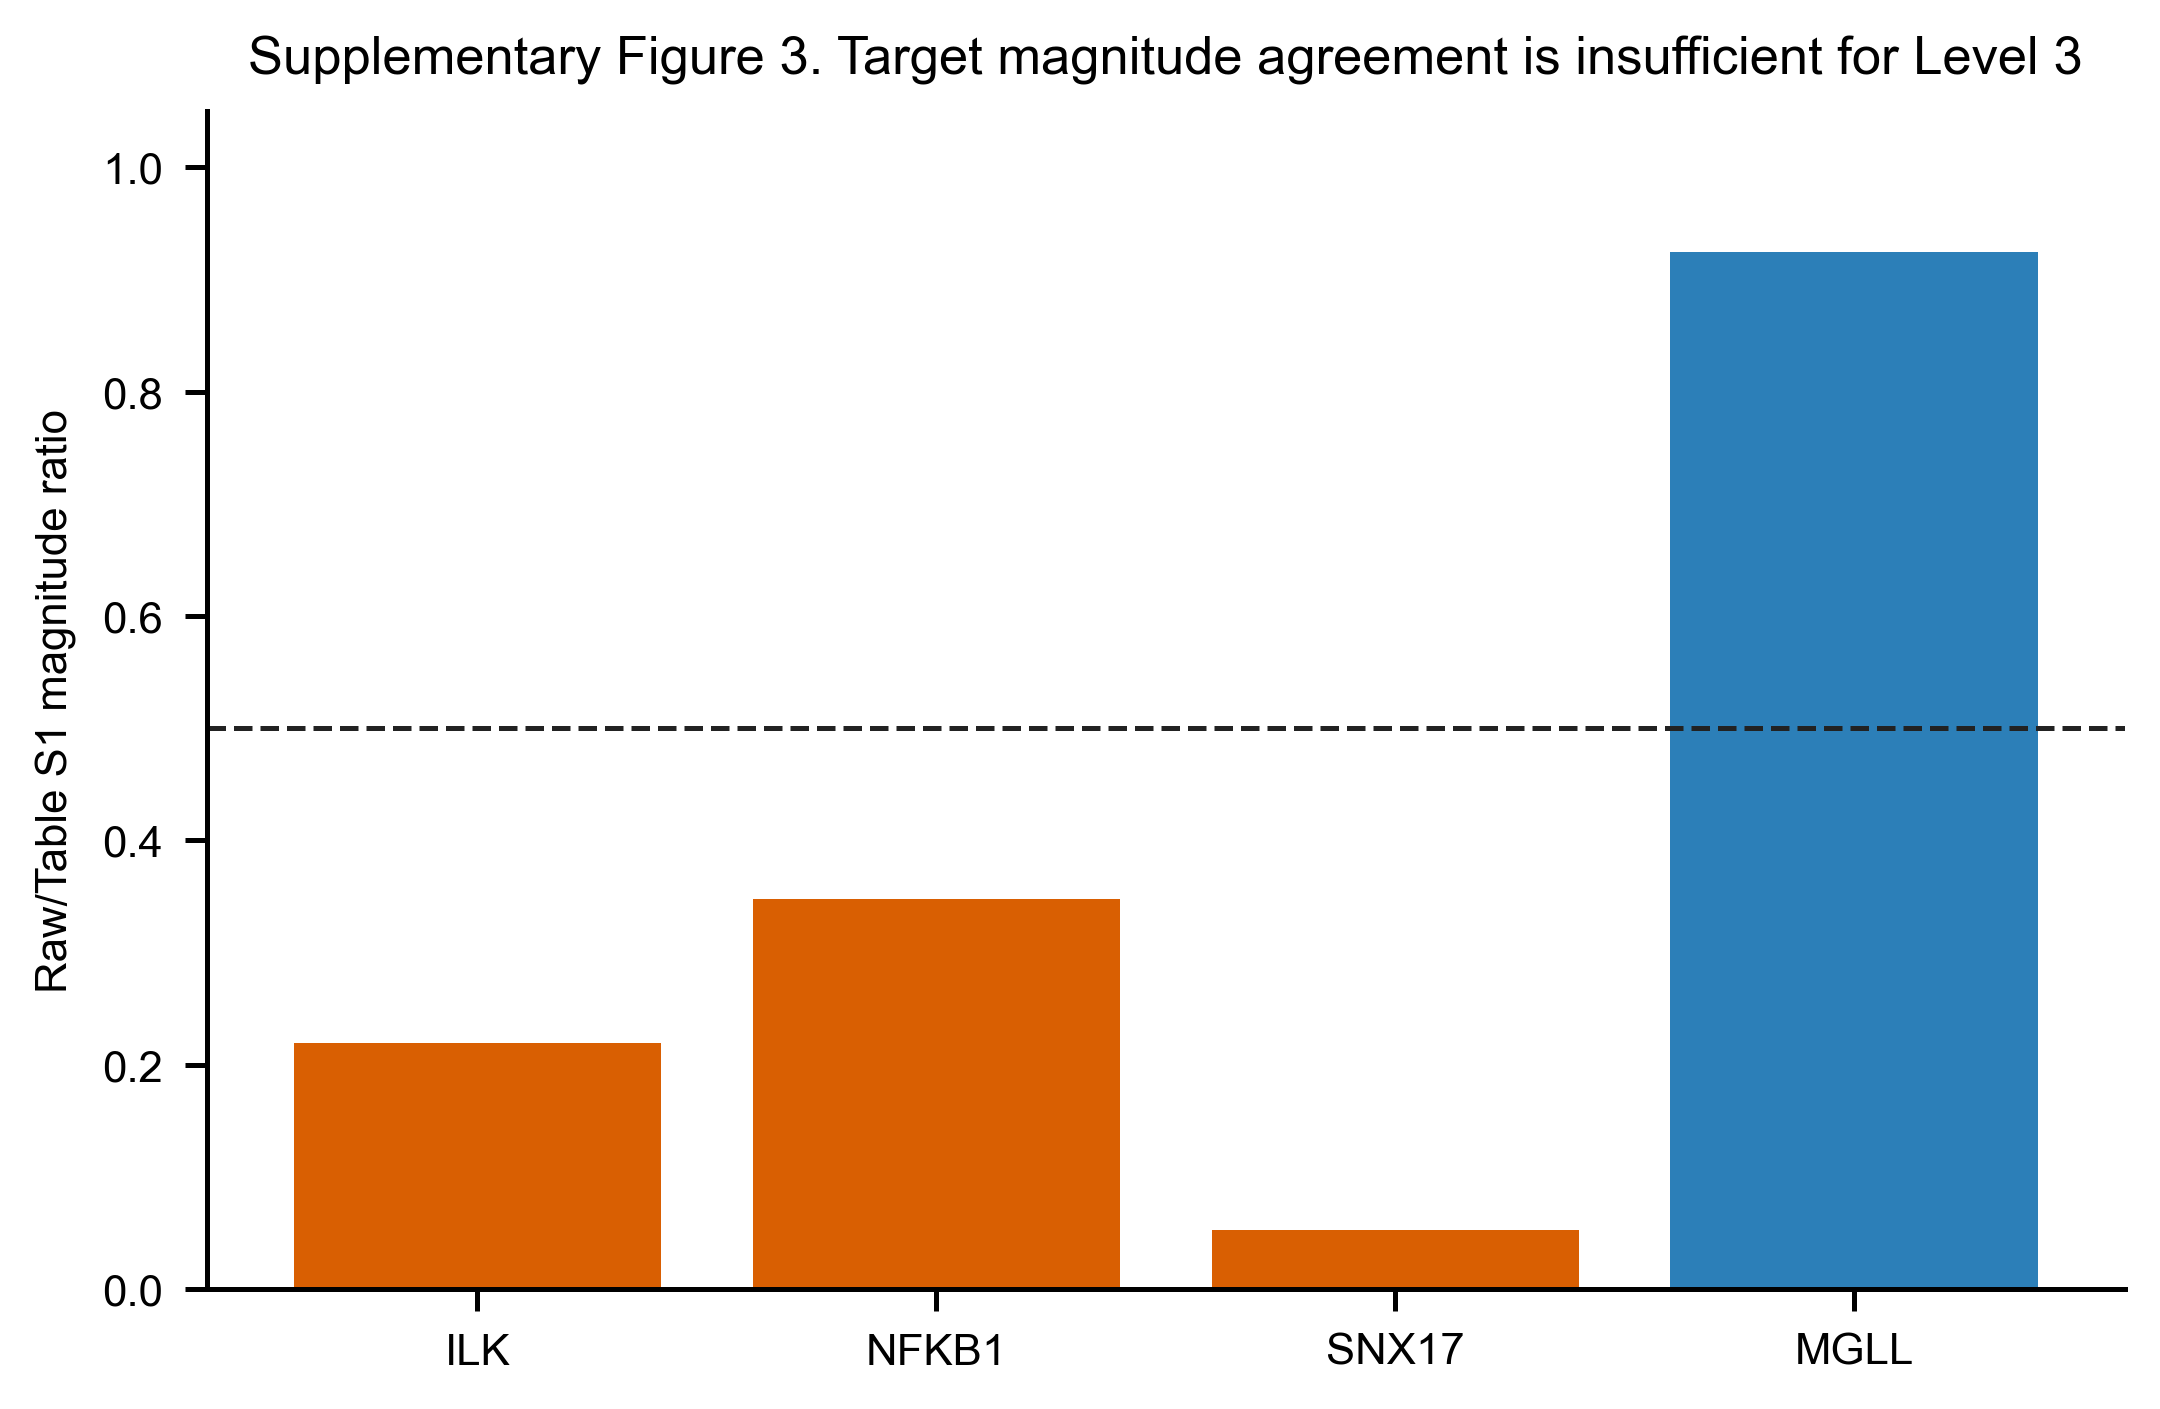
\includegraphics[width=0.82\linewidth]{suppfig4_target_magnitude.png}
\end{center}


\subsection*{Supplementary Note 6. GSE104896 mRNA boundary analysis}
GSE104896 was used only as an independent CTB mRNA boundary check. Among the 31675489 exosome-cargo decrease genes with non-zero paired CTB mRNA deltas, the positive fraction was 0.677 compared with a matched-null mean of 0.504. The mean log2 delta was 0.048 compared with matched-null mean 0.005. No CTD-mapped gene passed all-background BH-FDR < 0.05 in the donor-paired exact sign-flip model.

\subsection*{Supplementary Note 7. Alternative explanations and boundaries}
The manuscript does not claim a pure compartment-only effect. PMID 31675489 and PMID 37385330 differ in dose, exposure time, model, sample preparation, proteomic workflow and normalization. The evidence therefore supports compartment/readout/model-conditioned divergence. The claim would be strengthened by the author-level per-protein limma/FDR table for PMID 37385330 or by a same-sample matched cell-lysate versus extracellular-vesicle validation.

\subsection*{Supplementary Note 8. Reproducibility appendix}
\begin{itemize}[leftmargin=*]
\item \textbf{CTD scaffold.} The source-readiness scan used the local run \texttt{20260523T105644Z}, bounded to 2,000,000 non-comment CTD Chemical-Gene Interaction rows. Rows were retained only when they had a PubMed identifier, direct chemical-gene evidence, an \texttt{increases} or \texttt{decreases} direction in expression/activity action classes, a source-readiness pass flag and a chemical-to-gene orientation sentence. The orientation rule was heuristic and fail-closed: obvious gene/protein-to-chemical metabolism or activation sentences were excluded.
\item \textbf{BDE-47 null audit.} The cluster background used a 20-chemical row-count-nearest background and a 10,000-iteration BDE-47 sign-label permutation with seed 47. The permutation shuffled increase/decrease labels across BDE-47 gene row groups while preserving row counts per group and the overall BDE-47 sign balance.
\item \textbf{PMID 31675489.} The exosome-cargo block was mapped from CTD gene symbols to the PBDE47 supplement table; listed zero-FC values were retained as reported and floored only for log-scale display. Direction concordance was computed from the reported fold-change direction, not from floored display values.
\item \textbf{PMID 37385330 Table S1.} Cellular proteome contrasts were computed as \(\log_2(\mathrm{mean}_{\mathrm{BDE47,condition}}/\mathrm{mean}_{\mathrm{vehicle,matched\ time}})\) from positive Table S1 relative abundance values. No pseudocount was added for retained proteins. The six Table S1 BDE-47 dose-time conditions were 1~\microM{} 15 h, 5~\microM{} 15 h, 1~\microM{} 24 h, 5~\microM{} 24 h, 1~\microM{} 39 h and 5~\microM{} 39 h.
\item \textbf{DIA-NN pilot.} The raw-pilot source was MassIVE MSV000087870, BDE-47 5~\microM{}, 39 h versus vehicle 39 h. SCIEX WIFF/\texttt{.scan} files were converted in a Windows-compatible route to seven \texttt{.wiff.dia} inputs: three BDE-47 5~\microM{} 39 h files and four vehicle 39 h files. DIA-NN 1.8.1 library-free quantification used a human UniProt SwissProt FASTA downloaded on 2026-05-24, predicted library generation with \texttt{--fasta-search} and \texttt{--predictor}, and protein-group matrix output. The command structure was recorded as \texttt{DiaNN.exe --f <seven .wiff.dia inputs> --fasta <human SwissProt FASTA> --fasta-search --predictor --matrices --out report.tsv}; target extraction then used \texttt{report.pg\_matrix.tsv}. Missing or zero protein-group quantities were left missing for log2 summaries and were not imputed.
\item \textbf{Target statistics.} Target-level log2 deltas were computed from detected non-zero replicate protein-group quantities. Exact target-only permutation p-values were computed over detected replicate log2 abundances. These p-values were descriptive and were not interpreted as global proteome FDR or author-level limma/FDR.
\item \textbf{GSE104896.} CTB mRNA analysis used processed GEO expression records, platform-based probe-to-gene mapping and donor-paired BDE-47 versus vehicle deltas where pairing metadata were available. Background matching used selected-probe mean expression, expression standard deviation, paired-delta standard deviation and probe count. The gene-level boundary used donor-paired exact sign-flip testing with all-background Benjamini-Hochberg FDR.
\end{itemize}


\subsubsection*{Supplementary Figure 4. Cluster size versus seed count.}
\begin{center}
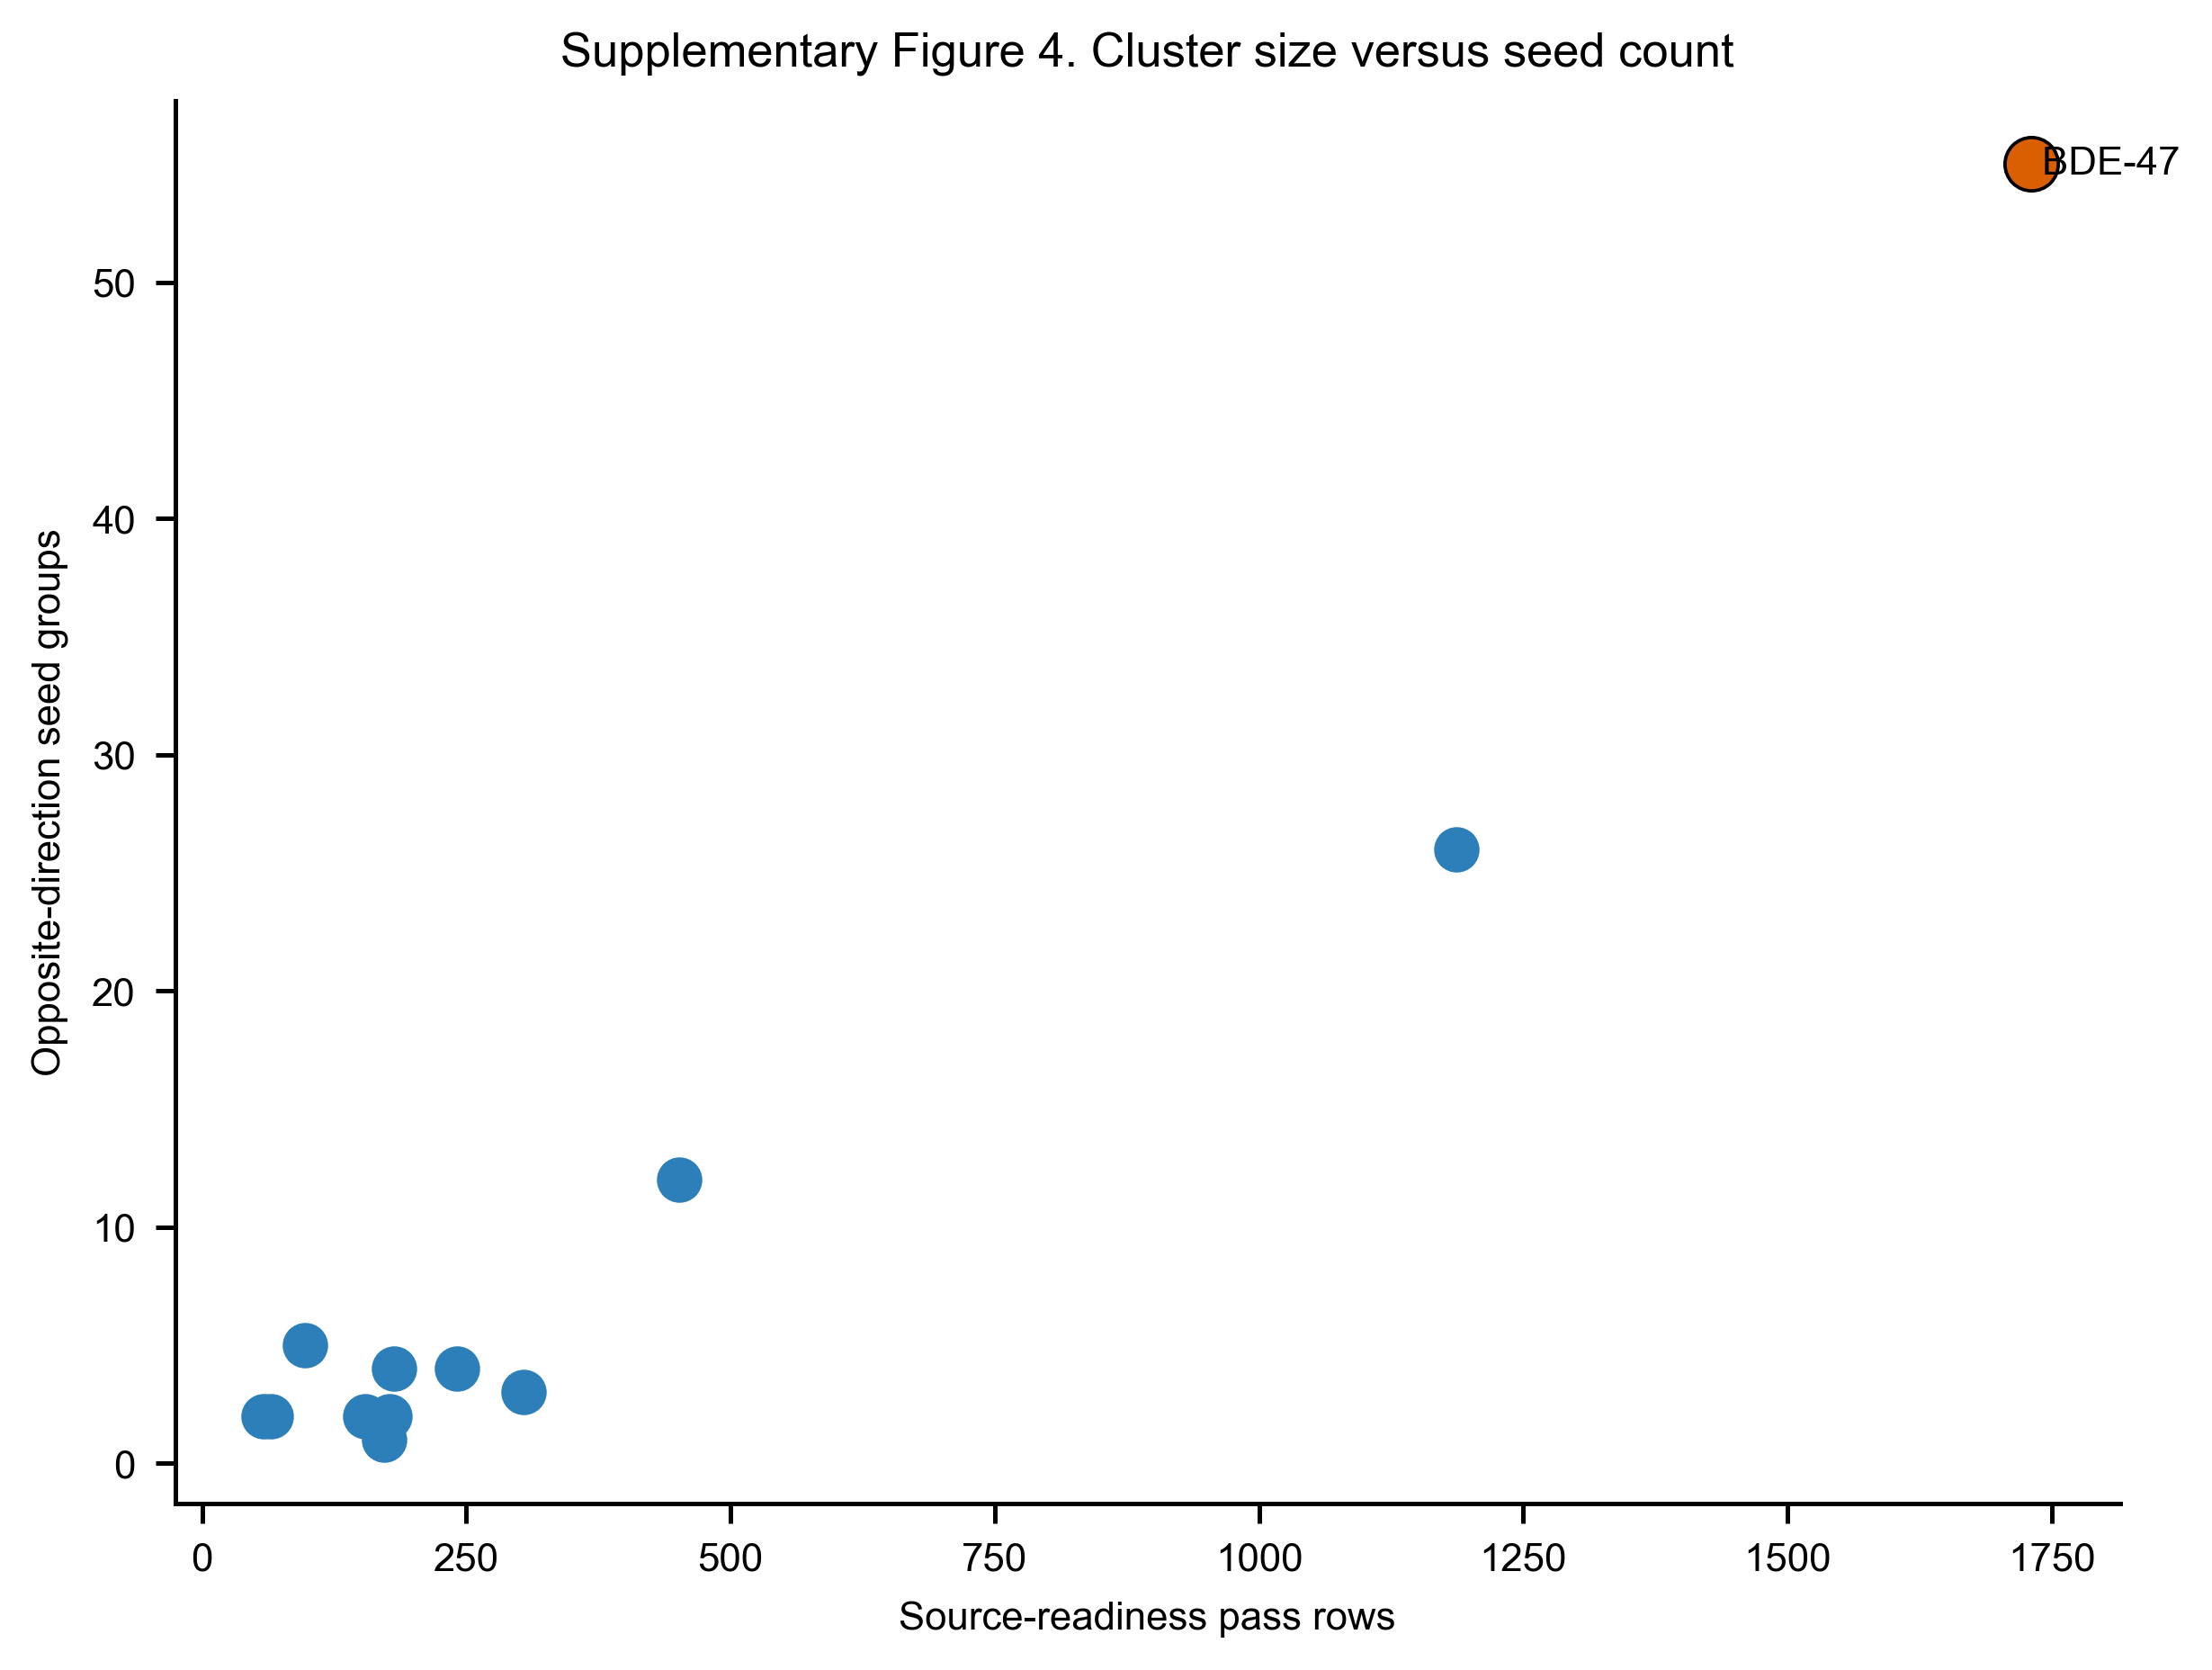
\includegraphics[width=0.82\linewidth]{suppfig3_cluster_background.png}
\end{center}


\subsection*{Supplementary Tables}
\begin{itemize}[leftmargin=*]
\item \textbf{Supplementary Table 1.} \texttt{protein\_selection\_tree.tsv} --- inclusion tree for ILK, NFKB1, SNX17 and supplementary MGLL.
\item \textbf{Supplementary Table 2.} \texttt{ctd\_cluster\_background\_audit.tsv} --- BDE-47 CTD cluster background audit.
\item \textbf{Supplementary Table 3.} \texttt{raw\_pilot\_vs\_table\_s1\_target\_qc.tsv} --- target-level raw-pilot versus Table S1 QC.
\item \textbf{Supplementary Table 4.} \texttt{raw\_pilot\_vs\_table\_s1\_global\_qc.tsv} --- gene-level pg-matrix versus Table S1 QC.
\item \textbf{Supplementary Table 5.} \texttt{proteome\_contrast\_evidence\_level\_gate.tsv} --- proteome contrast evidence-level gate.
\item \textbf{Supplementary Table 6.} \texttt{claim\_evidence\_boundary\_map.tsv} --- claim-evidence-boundary map.
\end{itemize}

\end{document}
